\documentclass[1p]{elsarticle_modified}
%\bibliographystyle{elsarticle-num}

%\usepackage[colorlinks]{hyperref}
%\usepackage{abbrmath_seonhwa} %\Abb, \Ascr, \Acal ,\Abf, \Afrak
\usepackage{amsfonts}
\usepackage{amssymb}
\usepackage{amsmath}
\usepackage{amsthm}
\usepackage{scalefnt}
\usepackage{amsbsy}
\usepackage{kotex}
\usepackage{caption}
\usepackage{subfig}
\usepackage{color}
\usepackage{graphicx}
\usepackage{xcolor} %% white, black, red, green, blue, cyan, magenta, yellow
\usepackage{float}
\usepackage{setspace}
\usepackage{hyperref}

\usepackage{tikz}
\usetikzlibrary{arrows}

\usepackage{multirow}
\usepackage{array} % fixed length table
\usepackage{hhline}

%%%%%%%%%%%%%%%%%%%%%
\makeatletter
\renewcommand*\env@matrix[1][\arraystretch]{%
	\edef\arraystretch{#1}%
	\hskip -\arraycolsep
	\let\@ifnextchar\new@ifnextchar
	\array{*\c@MaxMatrixCols c}}
\makeatother %https://tex.stackexchange.com/questions/14071/how-can-i-increase-the-line-spacing-in-a-matrix
%%%%%%%%%%%%%%%

\usepackage[normalem]{ulem}

\newcommand{\msout}[1]{\ifmmode\text{\sout{\ensuremath{#1}}}\else\sout{#1}\fi}
%SOURCE: \msout is \stkout macro in https://tex.stackexchange.com/questions/20609/strikeout-in-math-mode

\newcommand{\cancel}[1]{
	\ifmmode
	{\color{red}\msout{#1}}
	\else
	{\color{red}\sout{#1}}
	\fi
}

\newcommand{\add}[1]{
	{\color{blue}\uwave{#1}}
}

\newcommand{\replace}[2]{
	\ifmmode
	{\color{red}\msout{#1}}{\color{blue}\uwave{#2}}
	\else
	{\color{red}\sout{#1}}{\color{blue}\uwave{#2}}
	\fi
}

\newcommand{\Sol}{\mathcal{S}} %segment
\newcommand{\D}{D} %diagram
\newcommand{\A}{\mathcal{A}} %arc


%%%%%%%%%%%%%%%%%%%%%%%%%%%%%5 test

\def\sl{\operatorname{\textup{SL}}(2,\Cbb)}
\def\psl{\operatorname{\textup{PSL}}(2,\Cbb)}
\def\quan{\mkern 1mu \triangleright \mkern 1mu}

\theoremstyle{definition}
\newtheorem{thm}{Theorem}[section]
\newtheorem{prop}[thm]{Proposition}
\newtheorem{lem}[thm]{Lemma}
\newtheorem{ques}[thm]{Question}
\newtheorem{cor}[thm]{Corollary}
\newtheorem{defn}[thm]{Definition}
\newtheorem{exam}[thm]{Example}
\newtheorem{rmk}[thm]{Remark}
\newtheorem{alg}[thm]{Algorithm}

\newcommand{\I}{\sqrt{-1}}
\begin{document}

%\begin{frontmatter}
%
%\title{Boundary parabolic representations of knots up to 8 crossings}
%
%%% Group authors per affiliation:
%\author{Yunhi Cho} 
%\address{Department of Mathematics, University of Seoul, Seoul, Korea}
%\ead{yhcho@uos.ac.kr}
%
%
%\author{Seonhwa Kim} %\fnref{s_kim}}
%\address{Center for Geometry and Physics, Institute for Basic Science, Pohang, 37673, Korea}
%\ead{ryeona17@ibs.re.kr}
%
%\author{Hyuk Kim}
%\address{Department of Mathematical Sciences, Seoul National University, Seoul 08826, Korea}
%\ead{hyukkim@snu.ac.kr}
%
%\author{Seokbeom Yoon}
%\address{Department of Mathematical Sciences, Seoul National University, Seoul, 08826,  Korea}
%\ead{sbyoon15@snu.ac.kr}
%
%\begin{abstract}
%We find all boundary parabolic representation of knots up to 8 crossings.
%
%\end{abstract}
%\begin{keyword}
%    \MSC[2010] 57M25 
%\end{keyword}
%
%\end{frontmatter}

%\linenumbers
%\tableofcontents
%
\newcommand\colored[1]{\textcolor{white}{\rule[-0.35ex]{0.8em}{1.4ex}}\kern-0.8em\color{red} #1}%
%\newcommand\colored[1]{\textcolor{white}{ #1}\kern-2.17ex	\textcolor{white}{ #1}\kern-1.81ex	\textcolor{white}{ #1}\kern-2.15ex\color{red}#1	}

{\Large $\underline{11a_{239}~(K11a_{239})}$}

\setlength{\tabcolsep}{10pt}
\renewcommand{\arraystretch}{1.6}
\vspace{1cm}\begin{tabular}{m{100pt}>{\centering\arraybackslash}m{274pt}}
\multirow{5}{120pt}{
	\centering
	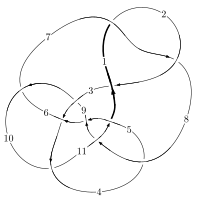
\includegraphics[width=112pt]{../../../GIT/diagram.site/Diagrams/png/488_11a_239.png}\\
\ \ \ A knot diagram\footnotemark}&
\allowdisplaybreaks
\textbf{Linearized knot diagam} \\
\cline{2-2}
 &
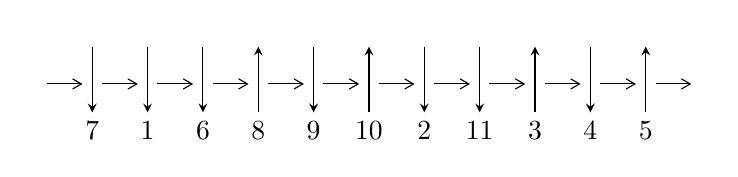
\begin{tikzpicture}[x=20pt, y=17pt]
	% nodes
	\node (C0) at (0, 0) {};
	\node (C1) at (1, 0) {};
	\node (C1U) at (1, +1) {};
	\node (C1D) at (1, -1) {7};

	\node (C2) at (2, 0) {};
	\node (C2U) at (2, +1) {};
	\node (C2D) at (2, -1) {1};

	\node (C3) at (3, 0) {};
	\node (C3U) at (3, +1) {};
	\node (C3D) at (3, -1) {6};

	\node (C4) at (4, 0) {};
	\node (C4U) at (4, +1) {};
	\node (C4D) at (4, -1) {8};

	\node (C5) at (5, 0) {};
	\node (C5U) at (5, +1) {};
	\node (C5D) at (5, -1) {9};

	\node (C6) at (6, 0) {};
	\node (C6U) at (6, +1) {};
	\node (C6D) at (6, -1) {10};

	\node (C7) at (7, 0) {};
	\node (C7U) at (7, +1) {};
	\node (C7D) at (7, -1) {2};

	\node (C8) at (8, 0) {};
	\node (C8U) at (8, +1) {};
	\node (C8D) at (8, -1) {11};

	\node (C9) at (9, 0) {};
	\node (C9U) at (9, +1) {};
	\node (C9D) at (9, -1) {3};

	\node (C10) at (10, 0) {};
	\node (C10U) at (10, +1) {};
	\node (C10D) at (10, -1) {4};

	\node (C11) at (11, 0) {};
	\node (C11U) at (11, +1) {};
	\node (C11D) at (11, -1) {5};
	\node (C12) at (12, 0) {};

	% arrows
	\draw[->,>={angle 60}]
	(C0) edge (C1) (C1) edge (C2) (C2) edge (C3) (C3) edge (C4) (C4) edge (C5) (C5) edge (C6) (C6) edge (C7) (C7) edge (C8) (C8) edge (C9) (C9) edge (C10) (C10) edge (C11) (C11) edge (C12) ;	\draw[->,>=stealth]
	(C1U) edge (C1D) (C2U) edge (C2D) (C3U) edge (C3D) (C4D) edge (C4U) (C5U) edge (C5D) (C6D) edge (C6U) (C7U) edge (C7D) (C8U) edge (C8D) (C9D) edge (C9U) (C10U) edge (C10D) (C11D) edge (C11U) ;
	\end{tikzpicture} \\
\hhline{~~} \\& 
\textbf{Solving Sequence} \\ \cline{2-2} 
 &
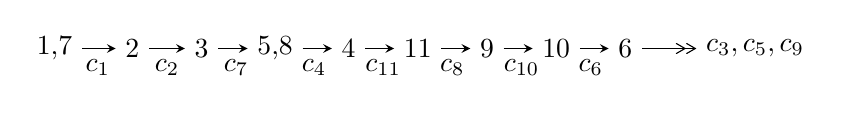
\begin{tikzpicture}[x=25pt, y=7pt]
	% node
	\node (A0) at (-1/8, 0) {1,7};
	\node (A1) at (1, 0) {2};
	\node (A2) at (2, 0) {3};
	\node (A3) at (49/16, 0) {5,8};
	\node (A4) at (33/8, 0) {4};
	\node (A5) at (41/8, 0) {11};
	\node (A6) at (49/8, 0) {9};
	\node (A7) at (57/8, 0) {10};
	\node (A8) at (65/8, 0) {6};
	\node (C1) at (1/2, -1) {$c_{1}$};
	\node (C2) at (3/2, -1) {$c_{2}$};
	\node (C3) at (5/2, -1) {$c_{7}$};
	\node (C4) at (29/8, -1) {$c_{4}$};
	\node (C5) at (37/8, -1) {$c_{11}$};
	\node (C6) at (45/8, -1) {$c_{8}$};
	\node (C7) at (53/8, -1) {$c_{10}$};
	\node (C8) at (61/8, -1) {$c_{6}$};
	\node (A9) at (10, 0) {$c_{3},c_{5},c_{9}$};

	% edge
	\draw[->,>=stealth]	
	(A0) edge (A1) (A1) edge (A2) (A2) edge (A3) (A3) edge (A4) (A4) edge (A5) (A5) edge (A6) (A6) edge (A7) (A7) edge (A8) ;
	\draw[->>,>={angle 60}]	
	(A8) edge (A9);
\end{tikzpicture} \\ 

\end{tabular} \\

\footnotetext{
The image of knot diagram is generated by the software ``\textbf{Draw programme}" developed by Andrew Bartholomew(\url{http://www.layer8.co.uk/maths/draw/index.htm\#Running-draw}), where we modified some parts for our purpose(\url{https://github.com/CATsTAILs/LinksPainter}).
}\phantom \\ \newline 
\centering \textbf{Ideals for irreducible components\footnotemark of $X_{\text{par}}$} 
 
\begin{align*}
I^u_{1}&=\langle 
3 u^{16}-18 u^{15}+\cdots+4 b+36,\;-11 u^{16}+64 u^{15}+\cdots+8 a-132,\;u^{17}-6 u^{16}+\cdots+28 u-8\rangle \\
I^u_{2}&=\langle 
- u^2 a+a u+b,\\
\phantom{I^u_{2}}&\phantom{= \langle  }4 u^5 a-9 u^6-4 u^4 a+19 u^5-4 u^3 a-7 u^4+8 u^2 a-30 u^3+8 a^2-12 a u+53 u^2+12 a-61 u+22,\\
\phantom{I^u_{2}}&\phantom{= \langle  }u^7-3 u^6+3 u^5+2 u^4-9 u^3+13 u^2-10 u+4\rangle \\
I^u_{3}&=\langle 
-2.57269\times10^{30} a^{7} u^{5}+1.10741\times10^{30} a^{6} u^{5}+\cdots-6.76928\times10^{31} a-1.39005\times10^{31},\\
\phantom{I^u_{3}}&\phantom{= \langle  }a^7 u^5-3 a^6 u^5+\cdots-8 a+4,\;u^6+u^5- u^4-2 u^3+u+1\rangle \\
I^u_{4}&=\langle 
29259 u^5 a^3+22409 u^5 a^2+\cdots+58215 a+25537,\;- u^5 a^3+u^5 a+\cdots+a^4+2 a,\\
\phantom{I^u_{4}}&\phantom{= \langle  }u^6+u^5- u^4-2 u^3+u+1\rangle \\
I^u_{5}&=\langle 
5 u^{21}- u^{20}+\cdots+2 b-5,\;22 u^{21}-27 u^{20}+\cdots+6 a+3,\\
\phantom{I^u_{5}}&\phantom{= \langle  }u^{22}-8 u^{20}+29 u^{18}-65 u^{16}+96 u^{14}-95 u^{12}+59 u^{10}-20 u^8+5 u^6-8 u^4+8 u^2-3\rangle \\
I^u_{6}&=\langle 
- u^5- u^4- u^2 a- a u+u^2+b+u+1,\;u^5 a+2 u^4 a- u^4-2 u^2 a- u^3+a^2- a u- u^2+2 u,\\
\phantom{I^u_{6}}&\phantom{= \langle  }u^6+u^5- u^4-2 u^3+u+1\rangle \\
I^u_{7}&=\langle 
- u^5+u^3+b- u,\;u^5-2 u^3+a+u,\;u^6- u^5- u^4+2 u^3- u+1\rangle \\
\\
I^v_{1}&=\langle 
a,\;b^2+b+1,\;v+1\rangle \\
\end{align*}
\raggedright * 8 irreducible components of $\dim_{\mathbb{C}}=0$, with total 145 representations.\\
\footnotetext{All coefficients of polynomials are rational numbers. But the coefficients are sometimes approximated in decimal forms when there is not enough margin.}
\newpage
\renewcommand{\arraystretch}{1}
\centering \section*{I. $I^u_{1}= \langle 3 u^{16}-18 u^{15}+\cdots+4 b+36,\;-11 u^{16}+64 u^{15}+\cdots+8 a-132,\;u^{17}-6 u^{16}+\cdots+28 u-8 \rangle$}
\flushleft \textbf{(i) Arc colorings}\\
\begin{tabular}{m{7pt} m{180pt} m{7pt} m{180pt} }
\flushright $a_{1}=$&$\begin{pmatrix}1\\0\end{pmatrix}$ \\
\flushright $a_{7}=$&$\begin{pmatrix}0\\u\end{pmatrix}$ \\
\flushright $a_{2}=$&$\begin{pmatrix}1\\u^2\end{pmatrix}$ \\
\flushright $a_{3}=$&$\begin{pmatrix}- u^2+1\\u^2\end{pmatrix}$ \\
\flushright $a_{5}=$&$\begin{pmatrix}\frac{11}{8} u^{16}-8 u^{15}+\cdots-\frac{89}{2} u+\frac{33}{2}\\-\frac{3}{4} u^{16}+\frac{9}{2} u^{15}+\cdots+26 u-9\end{pmatrix}$ \\
\flushright $a_{8}=$&$\begin{pmatrix}- u\\- u^3+u\end{pmatrix}$ \\
\flushright $a_{4}=$&$\begin{pmatrix}\frac{11}{8} u^{16}-\frac{15}{2} u^{15}+\cdots-\frac{65}{2} u+\frac{21}{2}\\-\frac{3}{4} u^{16}+2 u^{15}+\cdots-5 u^2+1\end{pmatrix}$ \\
\flushright $a_{11}=$&$\begin{pmatrix}-\frac{7}{8} u^{16}+\frac{21}{4} u^{15}+\cdots+19 u-\frac{13}{2}\\2 u^{16}-\frac{19}{2} u^{15}+\cdots-24 u+7\end{pmatrix}$ \\
\flushright $a_{9}=$&$\begin{pmatrix}\frac{1}{8} u^{16}-\frac{3}{2} u^{15}+\cdots-\frac{19}{2} u+\frac{7}{2}\\-\frac{3}{4} u^{16}+5 u^{15}+\cdots+28 u-11\end{pmatrix}$ \\
\flushright $a_{10}=$&$\begin{pmatrix}-\frac{9}{8} u^{16}+6 u^{15}+\cdots+\frac{45}{2} u-\frac{11}{2}\\-\frac{1}{4} u^{16}+2 u^{15}+\cdots+22 u-11\end{pmatrix}$ \\
\flushright $a_{6}=$&$\begin{pmatrix}-\frac{7}{8} u^{16}+\frac{13}{4} u^{15}+\cdots+2 u-\frac{1}{2}\\2 u^{15}-\frac{15}{2} u^{14}+\cdots+18 u-7\end{pmatrix}$\\ \flushright $a_{6}=$&$\begin{pmatrix}-\frac{7}{8} u^{16}+\frac{13}{4} u^{15}+\cdots+2 u-\frac{1}{2}\\2 u^{15}-\frac{15}{2} u^{14}+\cdots+18 u-7\end{pmatrix}$\\&\end{tabular}
\flushleft \textbf{(ii) Obstruction class $= -1$}\\~\\
\flushleft \textbf{(iii) Cusp Shapes $= -\frac{29}{2} u^{16}+72 u^{15}-\frac{209}{2} u^{14}-120 u^{13}+\frac{1253}{2} u^{12}-780 u^{11}-\frac{287}{2} u^{10}+1656 u^9-\frac{4241}{2} u^8+703 u^7+\frac{2779}{2} u^6-2264 u^5+\frac{3031}{2} u^4-319 u^3-255 u^2+226 u-62$}\\~\\
\newpage\renewcommand{\arraystretch}{1}
\flushleft \textbf{(iv) u-Polynomials at the component}\newline \\
\begin{tabular}{m{50pt}|m{274pt}}
Crossings & \hspace{64pt}u-Polynomials at each crossing \\
\hline $$\begin{aligned}c_{1},c_{7}\end{aligned}$$&$\begin{aligned}
&u^{17}-6 u^{16}+\cdots+28 u-8
\end{aligned}$\\
\hline $$\begin{aligned}c_{2}\end{aligned}$$&$\begin{aligned}
&u^{17}+10 u^{16}+\cdots+208 u+64
\end{aligned}$\\
\hline $$\begin{aligned}c_{3},c_{8}\end{aligned}$$&$\begin{aligned}
&u^{17}-13 u^{16}+\cdots+259 u-47
\end{aligned}$\\
\hline $$\begin{aligned}c_{4},c_{6},c_{9}\\c_{11}\end{aligned}$$&$\begin{aligned}
&u^{17}- u^{16}+\cdots+u-1
\end{aligned}$\\
\hline $$\begin{aligned}c_{5},c_{10}\end{aligned}$$&$\begin{aligned}
&u^{17}+2 u^{16}+\cdots- u+4
\end{aligned}$\\
\hline
\end{tabular}\\~\\
\newpage\renewcommand{\arraystretch}{1}
\flushleft \textbf{(v) Riley Polynomials at the component}\newline \\
\begin{tabular}{m{50pt}|m{274pt}}
Crossings & \hspace{64pt}Riley Polynomials at each crossing \\
\hline $$\begin{aligned}c_{1},c_{7}\end{aligned}$$&$\begin{aligned}
&y^{17}-10 y^{16}+\cdots+208 y-64
\end{aligned}$\\
\hline $$\begin{aligned}c_{2}\end{aligned}$$&$\begin{aligned}
&y^{17}-6 y^{16}+\cdots+47360 y-4096
\end{aligned}$\\
\hline $$\begin{aligned}c_{3},c_{8}\end{aligned}$$&$\begin{aligned}
&y^{17}-13 y^{16}+\cdots-7555 y-2209
\end{aligned}$\\
\hline $$\begin{aligned}c_{4},c_{6},c_{9}\\c_{11}\end{aligned}$$&$\begin{aligned}
&y^{17}-5 y^{16}+\cdots+21 y-1
\end{aligned}$\\
\hline $$\begin{aligned}c_{5},c_{10}\end{aligned}$$&$\begin{aligned}
&y^{17}-12 y^{16}+\cdots+177 y-16
\end{aligned}$\\
\hline
\end{tabular}\\~\\
\newpage\flushleft \textbf{(vi) Complex Volumes and Cusp Shapes}
$$\begin{array}{c|c|c}  
\text{Solutions to }I^u_{1}& \I (\text{vol} + \sqrt{-1}CS) & \text{Cusp shape}\\
 \hline 
\begin{aligned}
u &= \phantom{-}0.334231 + 0.945289 I \\
a &= \phantom{-}1.186990 + 0.667740 I \\
b &= -1.11552 - 1.11726 I\end{aligned}
 & -1.10093 + 13.85920 I & -2.71296 - 7.57439 I \\ \hline\begin{aligned}
u &= \phantom{-}0.334231 - 0.945289 I \\
a &= \phantom{-}1.186990 - 0.667740 I \\
b &= -1.11552 + 1.11726 I\end{aligned}
 & -1.10093 - 13.85920 I & -2.71296 + 7.57439 I \\ \hline\begin{aligned}
u &= \phantom{-}0.788176 + 0.924452 I \\
a &= -0.655874 - 0.649894 I \\
b &= \phantom{-}1.016290 + 0.314455 I\end{aligned}
 & \phantom{-}2.41973 + 2.94950 I & \phantom{-}2.91048 - 5.30771 I \\ \hline\begin{aligned}
u &= \phantom{-}0.788176 - 0.924452 I \\
a &= -0.655874 + 0.649894 I \\
b &= \phantom{-}1.016290 - 0.314455 I\end{aligned}
 & \phantom{-}2.41973 - 2.94950 I & \phantom{-}2.91048 + 5.30771 I \\ \hline\begin{aligned}
u &= \phantom{-}0.857122 + 0.870195 I \\
a &= \phantom{-}1.129770 + 0.148811 I \\
b &= -1.086350 + 0.571276 I\end{aligned}
 & \phantom{-}2.21297 - 9.35015 I & -0.11785 + 9.82632 I \\ \hline\begin{aligned}
u &= \phantom{-}0.857122 - 0.870195 I \\
a &= \phantom{-}1.129770 - 0.148811 I \\
b &= -1.086350 - 0.571276 I\end{aligned}
 & \phantom{-}2.21297 + 9.35015 I & -0.11785 - 9.82632 I \\ \hline\begin{aligned}
u &= \phantom{-}0.337237 + 0.670381 I \\
a &= -1.111840 + 0.085153 I \\
b &= \phantom{-}0.766763 + 0.185332 I\end{aligned}
 & \phantom{-}1.74054 + 0.98669 I & \phantom{-}3.14210 - 1.82725 I \\ \hline\begin{aligned}
u &= \phantom{-}0.337237 - 0.670381 I \\
a &= -1.111840 - 0.085153 I \\
b &= \phantom{-}0.766763 - 0.185332 I\end{aligned}
 & \phantom{-}1.74054 - 0.98669 I & \phantom{-}3.14210 + 1.82725 I \\ \hline\begin{aligned}
u &= \phantom{-}1.164700 + 0.502631 I \\
a &= \phantom{-}0.659288 + 0.927604 I \\
b &= -0.659915 + 0.384127 I\end{aligned}
 & -0.77068 - 5.56913 I & -2.33811 + 7.26294 I \\ \hline\begin{aligned}
u &= \phantom{-}1.164700 - 0.502631 I \\
a &= \phantom{-}0.659288 - 0.927604 I \\
b &= -0.659915 - 0.384127 I\end{aligned}
 & -0.77068 + 5.56913 I & -2.33811 - 7.26294 I\\
 \hline 
 \end{array}$$\newpage$$\begin{array}{c|c|c}  
\text{Solutions to }I^u_{1}& \I (\text{vol} + \sqrt{-1}CS) & \text{Cusp shape}\\
 \hline 
\begin{aligned}
u &= \phantom{-}1.187760 + 0.627012 I \\
a &= -1.63439 - 0.99047 I \\
b &= \phantom{-}1.13230 - 1.24110 I\end{aligned}
 & -3.7013 - 19.5737 I & -5.36728 + 10.75666 I \\ \hline\begin{aligned}
u &= \phantom{-}1.187760 - 0.627012 I \\
a &= -1.63439 + 0.99047 I \\
b &= \phantom{-}1.13230 + 1.24110 I\end{aligned}
 & -3.7013 + 19.5737 I & -5.36728 - 10.75666 I \\ \hline\begin{aligned}
u &= -1.340970 + 0.177838 I \\
a &= \phantom{-}0.340570 - 0.263792 I \\
b &= \phantom{-}0.885606 - 1.042740 I\end{aligned}
 & -6.89672 - 10.17430 I & -7.93890 + 7.26215 I \\ \hline\begin{aligned}
u &= -1.340970 - 0.177838 I \\
a &= \phantom{-}0.340570 + 0.263792 I \\
b &= \phantom{-}0.885606 + 1.042740 I\end{aligned}
 & -6.89672 + 10.17430 I & -7.93890 - 7.26215 I \\ \hline\begin{aligned}
u &= \phantom{-}1.46179\phantom{ +0.000000I} \\
a &= \phantom{-}0.501964\phantom{ +0.000000I} \\
b &= \phantom{-}0.338845\phantom{ +0.000000I}\end{aligned}
 & -7.70589\phantom{ +0.000000I} & -19.1410\phantom{ +0.000000I} \\ \hline\begin{aligned}
u &= -0.515829\phantom{ +0.000000I} \\
a &= -0.663529\phantom{ +0.000000I} \\
b &= -0.518819\phantom{ +0.000000I}\end{aligned}
 & -1.37384\phantom{ +0.000000I} & -7.65930\phantom{ +0.000000I} \\ \hline\begin{aligned}
u &= -1.60248\phantom{ +0.000000I} \\
a &= -0.167458\phantom{ +0.000000I} \\
b &= -0.698369\phantom{ +0.000000I}\end{aligned}
 & -6.69142\phantom{ +0.000000I} & \phantom{-}13.6450\phantom{ +0.000000I}\\
 \hline 
 \end{array}$$\newpage\newpage\renewcommand{\arraystretch}{1}
\centering \section*{II. $I^u_{2}= \langle - u^2 a+a u+b,\;4 u^5 a-9 u^6+\cdots+12 a+22,\;u^7-3 u^6+3 u^5+2 u^4-9 u^3+13 u^2-10 u+4 \rangle$}
\flushleft \textbf{(i) Arc colorings}\\
\begin{tabular}{m{7pt} m{180pt} m{7pt} m{180pt} }
\flushright $a_{1}=$&$\begin{pmatrix}1\\0\end{pmatrix}$ \\
\flushright $a_{7}=$&$\begin{pmatrix}0\\u\end{pmatrix}$ \\
\flushright $a_{2}=$&$\begin{pmatrix}1\\u^2\end{pmatrix}$ \\
\flushright $a_{3}=$&$\begin{pmatrix}- u^2+1\\u^2\end{pmatrix}$ \\
\flushright $a_{5}=$&$\begin{pmatrix}a\\u^2 a- a u\end{pmatrix}$ \\
\flushright $a_{8}=$&$\begin{pmatrix}- u\\- u^3+u\end{pmatrix}$ \\
\flushright $a_{4}=$&$\begin{pmatrix}u^3 a- u^2 a+a\\u^5 a- u^4 a- u^3 a+2 u^2 a- a u\end{pmatrix}$ \\
\flushright $a_{11}=$&$\begin{pmatrix}-\frac{1}{2} u^6 a-\frac{1}{2} u^6+\cdots+2 a+\frac{3}{2}\\u^6 a+\frac{1}{2} u^6+\cdots-2 a+\frac{3}{2} u\end{pmatrix}$ \\
\flushright $a_{9}=$&$\begin{pmatrix}u^6-\frac{3}{2} u^5+\cdots+a-\frac{1}{2}\\-\frac{1}{2} u^6+\frac{1}{2} u^5+\cdots+a u-\frac{1}{2} u\end{pmatrix}$ \\
\flushright $a_{10}=$&$\begin{pmatrix}-\frac{1}{2} u^6+u^5+\cdots+a+\frac{3}{2}\\\frac{1}{2} u^6-\frac{1}{2} u^5+\cdots+a u+\frac{3}{2} u\end{pmatrix}$ \\
\flushright $a_{6}=$&$\begin{pmatrix}\frac{1}{2} u^6 a-\frac{1}{4} u^6+\cdots-\frac{13}{4} u+\frac{3}{2}\\- u^5 a+u^6+\cdots-2 a-3\end{pmatrix}$\\ \flushright $a_{6}=$&$\begin{pmatrix}\frac{1}{2} u^6 a-\frac{1}{4} u^6+\cdots-\frac{13}{4} u+\frac{3}{2}\\- u^5 a+u^6+\cdots-2 a-3\end{pmatrix}$\\&\end{tabular}
\flushleft \textbf{(ii) Obstruction class $= -1$}\\~\\
\flushleft \textbf{(iii) Cusp Shapes $= 7 u^6-10 u^5- u^4+26 u^3-27 u^2+16 u+2$}\\~\\
\newpage\renewcommand{\arraystretch}{1}
\flushleft \textbf{(iv) u-Polynomials at the component}\newline \\
\begin{tabular}{m{50pt}|m{274pt}}
Crossings & \hspace{64pt}u-Polynomials at each crossing \\
\hline $$\begin{aligned}c_{1},c_{7}\end{aligned}$$&$\begin{aligned}
&(u^7-3 u^6+3 u^5+2 u^4-9 u^3+13 u^2-10 u+4)^2
\end{aligned}$\\
\hline $$\begin{aligned}c_{2}\end{aligned}$$&$\begin{aligned}
&(u^7+3 u^6+3 u^5-7 u^3+5 u^2-4 u+16)^2
\end{aligned}$\\
\hline $$\begin{aligned}c_{3},c_{8}\end{aligned}$$&$\begin{aligned}
&u^{14}-15 u^{13}+\cdots-1309 u+187
\end{aligned}$\\
\hline $$\begin{aligned}c_{4},c_{6},c_{9}\\c_{11}\end{aligned}$$&$\begin{aligned}
&u^{14}+u^{13}+\cdots+4 u+1
\end{aligned}$\\
\hline $$\begin{aligned}c_{5},c_{10}\end{aligned}$$&$\begin{aligned}
&(u^7- u^6+u^5- u^4+u^3+u-1)^2
\end{aligned}$\\
\hline
\end{tabular}\\~\\
\newpage\renewcommand{\arraystretch}{1}
\flushleft \textbf{(v) Riley Polynomials at the component}\newline \\
\begin{tabular}{m{50pt}|m{274pt}}
Crossings & \hspace{64pt}Riley Polynomials at each crossing \\
\hline $$\begin{aligned}c_{1},c_{7}\end{aligned}$$&$\begin{aligned}
&(y^7-3 y^6+3 y^5-7 y^3-5 y^2-4 y-16)^2
\end{aligned}$\\
\hline $$\begin{aligned}c_{2}\end{aligned}$$&$\begin{aligned}
&(y^7-3 y^6-5 y^5-80 y^4-71 y^3+31 y^2-144 y-256)^2
\end{aligned}$\\
\hline $$\begin{aligned}c_{3},c_{8}\end{aligned}$$&$\begin{aligned}
&y^{14}-3 y^{13}+\cdots-5797 y+34969
\end{aligned}$\\
\hline $$\begin{aligned}c_{4},c_{6},c_{9}\\c_{11}\end{aligned}$$&$\begin{aligned}
&y^{14}-3 y^{13}+\cdots-2 y+1
\end{aligned}$\\
\hline $$\begin{aligned}c_{5},c_{10}\end{aligned}$$&$\begin{aligned}
&(y^7+y^6+y^5+3 y^4+y^3+y-1)^2
\end{aligned}$\\
\hline
\end{tabular}\\~\\
\newpage\flushleft \textbf{(vi) Complex Volumes and Cusp Shapes}
$$\begin{array}{c|c|c}  
\text{Solutions to }I^u_{2}& \I (\text{vol} + \sqrt{-1}CS) & \text{Cusp shape}\\
 \hline 
\begin{aligned}
u &= \phantom{-}0.814935 + 0.691474 I \\
a &= \phantom{-}0.818477 + 1.080010 I \\
b &= -0.985169 - 0.322797 I\end{aligned}
 & \phantom{-}4.60437 - 2.63118 I & \phantom{-}2.98391 + 3.36378 I \\ \hline\begin{aligned}
u &= \phantom{-}0.814935 + 0.691474 I \\
a &= -1.56532 - 0.18032 I \\
b &= \phantom{-}1.063050 - 0.568346 I\end{aligned}
 & \phantom{-}4.60437 - 2.63118 I & \phantom{-}2.98391 + 3.36378 I \\ \hline\begin{aligned}
u &= \phantom{-}0.814935 - 0.691474 I \\
a &= \phantom{-}0.818477 - 1.080010 I \\
b &= -0.985169 + 0.322797 I\end{aligned}
 & \phantom{-}4.60437 + 2.63118 I & \phantom{-}2.98391 - 3.36378 I \\ \hline\begin{aligned}
u &= \phantom{-}0.814935 - 0.691474 I \\
a &= -1.56532 + 0.18032 I \\
b &= \phantom{-}1.063050 + 0.568346 I\end{aligned}
 & \phantom{-}4.60437 + 2.63118 I & \phantom{-}2.98391 - 3.36378 I \\ \hline\begin{aligned}
u &= \phantom{-}0.244291 + 1.049540 I \\
a &= -1.068000 - 0.437680 I \\
b &= \phantom{-}1.13868 + 1.13618 I\end{aligned}
 & \phantom{-}0.04250 + 5.03576 I & -2.7810 - 16.4347 I \\ \hline\begin{aligned}
u &= \phantom{-}0.244291 + 1.049540 I \\
a &= \phantom{-}0.330014 + 0.179733 I \\
b &= -0.327975 - 0.408300 I\end{aligned}
 & \phantom{-}0.04250 + 5.03576 I & -2.7810 - 16.4347 I \\ \hline\begin{aligned}
u &= \phantom{-}0.244291 - 1.049540 I \\
a &= -1.068000 + 0.437680 I \\
b &= \phantom{-}1.13868 - 1.13618 I\end{aligned}
 & \phantom{-}0.04250 - 5.03576 I & -2.7810 + 16.4347 I \\ \hline\begin{aligned}
u &= \phantom{-}0.244291 - 1.049540 I \\
a &= \phantom{-}0.330014 - 0.179733 I \\
b &= -0.327975 + 0.408300 I\end{aligned}
 & \phantom{-}0.04250 - 5.03576 I & -2.7810 + 16.4347 I \\ \hline\begin{aligned}
u &= \phantom{-}1.229510 + 0.632474 I \\
a &= -0.783908 - 0.339718 I \\
b &= \phantom{-}0.405865 - 0.683351 I\end{aligned}
 & -2.94764 - 10.98550 I & -7.63392 + 11.66372 I \\ \hline\begin{aligned}
u &= \phantom{-}1.229510 + 0.632474 I \\
a &= \phantom{-}1.43734 + 1.01814 I \\
b &= -1.10890 + 1.20639 I\end{aligned}
 & -2.94764 - 10.98550 I & -7.63392 + 11.66372 I\\
 \hline 
 \end{array}$$\newpage$$\begin{array}{c|c|c}  
\text{Solutions to }I^u_{2}& \I (\text{vol} + \sqrt{-1}CS) & \text{Cusp shape}\\
 \hline 
\begin{aligned}
u &= \phantom{-}1.229510 - 0.632474 I \\
a &= -0.783908 + 0.339718 I \\
b &= \phantom{-}0.405865 + 0.683351 I\end{aligned}
 & -2.94764 + 10.98550 I & -7.63392 - 11.66372 I \\ \hline\begin{aligned}
u &= \phantom{-}1.229510 - 0.632474 I \\
a &= \phantom{-}1.43734 - 1.01814 I \\
b &= -1.10890 - 1.20639 I\end{aligned}
 & -2.94764 + 10.98550 I & -7.63392 - 11.66372 I \\ \hline\begin{aligned}
u &= -1.57747\phantom{ +0.000000I} \\
a &= -0.168609 + 0.061232 I \\
b &= -0.685543 + 0.248960 I\end{aligned}
 & -6.68831\phantom{ +0.000000I} & \phantom{-}6.86200\phantom{ +0.000000I} \\ \hline\begin{aligned}
u &= -1.57747\phantom{ +0.000000I} \\
a &= -0.168609 - 0.061232 I \\
b &= -0.685543 - 0.248960 I\end{aligned}
 & -6.68831\phantom{ +0.000000I} & \phantom{-}6.86200\phantom{ +0.000000I}\\
 \hline 
 \end{array}$$\newpage\newpage\renewcommand{\arraystretch}{1}
\centering \section*{III. $I^u_{3}= \langle -2.57\times10^{30} a^{7} u^{5}+1.11\times10^{30} a^{6} u^{5}+\cdots-6.77\times10^{31} a-1.39\times10^{31},\;a^7 u^5-3 a^6 u^5+\cdots-8 a+4,\;u^6+u^5- u^4-2 u^3+u+1 \rangle$}
\flushleft \textbf{(i) Arc colorings}\\
\begin{tabular}{m{7pt} m{180pt} m{7pt} m{180pt} }
\flushright $a_{1}=$&$\begin{pmatrix}1\\0\end{pmatrix}$ \\
\flushright $a_{7}=$&$\begin{pmatrix}0\\u\end{pmatrix}$ \\
\flushright $a_{2}=$&$\begin{pmatrix}1\\u^2\end{pmatrix}$ \\
\flushright $a_{3}=$&$\begin{pmatrix}- u^2+1\\u^2\end{pmatrix}$ \\
\flushright $a_{5}=$&$\begin{pmatrix}a\\0.0725908 a^{7} u^{5}-0.0312466 a^{6} u^{5}+\cdots+1.91001 a+0.392216\end{pmatrix}$ \\
\flushright $a_{8}=$&$\begin{pmatrix}- u\\- u^3+u\end{pmatrix}$ \\
\flushright $a_{4}=$&$\begin{pmatrix}-0.0137916 a^{7} u^{5}+0.00218527 a^{6} u^{5}+\cdots+0.411608 a+0.495146\\0.151420 a^{7} u^{5}-0.00837117 a^{6} u^{5}+\cdots+2.66136 a+0.605770\end{pmatrix}$ \\
\flushright $a_{11}=$&$\begin{pmatrix}0.00470703 a^{7} u^{5}-0.00280449 a^{6} u^{5}+\cdots+0.181900 a+0.413915\\-0.103428 a^{7} u^{5}+0.0229172 a^{6} u^{5}+\cdots+1.71283 a-1.57617\end{pmatrix}$ \\
\flushright $a_{9}=$&$\begin{pmatrix}0.142900 a^{7} u^{5}-0.162959 a^{6} u^{5}+\cdots-0.921925 a+1.11192\\-0.0326497 a^{7} u^{5}-0.0359075 a^{6} u^{5}+\cdots+3.38577 a-1.09902\end{pmatrix}$ \\
\flushright $a_{10}=$&$\begin{pmatrix}0.138594 a^{7} u^{5}-0.138648 a^{6} u^{5}+\cdots-1.12523 a+1.42701\\-0.00903181 a^{7} u^{5}-0.0141319 a^{6} u^{5}+\cdots+3.74823 a-0.965404\end{pmatrix}$ \\
\flushright $a_{6}=$&$\begin{pmatrix}0.0782518 a^{7} u^{5}-0.0823113 a^{6} u^{5}+\cdots+0.426516 a-1.12444\\0.0398061 a^{7} u^{5}+0.0659338 a^{6} u^{5}+\cdots-2.81464 a+1.61215\end{pmatrix}$\\ \flushright $a_{6}=$&$\begin{pmatrix}0.0782518 a^{7} u^{5}-0.0823113 a^{6} u^{5}+\cdots+0.426516 a-1.12444\\0.0398061 a^{7} u^{5}+0.0659338 a^{6} u^{5}+\cdots-2.81464 a+1.61215\end{pmatrix}$\\&\end{tabular}
\flushleft \textbf{(ii) Obstruction class $= -1$}\\~\\
\flushleft \textbf{(iii) Cusp Shapes $= -\frac{4371177550733369341379808}{37338217638487684273785061} a^7 u^5-\frac{8613150463936407409230296}{37338217638487684273785061} a^6 u^5+\cdots-\frac{483487231400196111720296296}{37338217638487684273785061} a-\frac{520800134167026485786802942}{37338217638487684273785061}$}\\~\\
\newpage\renewcommand{\arraystretch}{1}
\flushleft \textbf{(iv) u-Polynomials at the component}\newline \\
\begin{tabular}{m{50pt}|m{274pt}}
Crossings & \hspace{64pt}u-Polynomials at each crossing \\
\hline $$\begin{aligned}c_{1},c_{7}\end{aligned}$$&$\begin{aligned}
&(u^6+u^5- u^4-2 u^3+u+1)^8
\end{aligned}$\\
\hline $$\begin{aligned}c_{2}\end{aligned}$$&$\begin{aligned}
&(u^6+3 u^5+5 u^4+4 u^3+2 u^2+u+1)^8
\end{aligned}$\\
\hline $$\begin{aligned}c_{3},c_{8}\end{aligned}$$&$\begin{aligned}
&(u^4+u^3-2 u+1)^{12}
\end{aligned}$\\
\hline $$\begin{aligned}c_{4},c_{6},c_{9}\\c_{11}\end{aligned}$$&$\begin{aligned}
&u^{48}- u^{47}+\cdots+258 u+67
\end{aligned}$\\
\hline $$\begin{aligned}c_{5},c_{10}\end{aligned}$$&$\begin{aligned}
&(u^{24}- u^{23}+\cdots-148 u+43)^{2}
\end{aligned}$\\
\hline
\end{tabular}\\~\\
\newpage\renewcommand{\arraystretch}{1}
\flushleft \textbf{(v) Riley Polynomials at the component}\newline \\
\begin{tabular}{m{50pt}|m{274pt}}
Crossings & \hspace{64pt}Riley Polynomials at each crossing \\
\hline $$\begin{aligned}c_{1},c_{7}\end{aligned}$$&$\begin{aligned}
&(y^6-3 y^5+5 y^4-4 y^3+2 y^2- y+1)^8
\end{aligned}$\\
\hline $$\begin{aligned}c_{2}\end{aligned}$$&$\begin{aligned}
&(y^6+y^5+5 y^4+6 y^2+3 y+1)^8
\end{aligned}$\\
\hline $$\begin{aligned}c_{3},c_{8}\end{aligned}$$&$\begin{aligned}
&(y^4- y^3+6 y^2-4 y+1)^{12}
\end{aligned}$\\
\hline $$\begin{aligned}c_{4},c_{6},c_{9}\\c_{11}\end{aligned}$$&$\begin{aligned}
&y^{48}+21 y^{47}+\cdots+251016 y+4489
\end{aligned}$\\
\hline $$\begin{aligned}c_{5},c_{10}\end{aligned}$$&$\begin{aligned}
&(y^{24}-21 y^{23}+\cdots-20872 y+1849)^{2}
\end{aligned}$\\
\hline
\end{tabular}\\~\\
\newpage\flushleft \textbf{(vi) Complex Volumes and Cusp Shapes}
$$\begin{array}{c|c|c}  
\text{Solutions to }I^u_{3}& \I (\text{vol} + \sqrt{-1}CS) & \text{Cusp shape}\\
 \hline 
\begin{aligned}
u &= \phantom{-}1.002190 + 0.295542 I \\
a &= -0.457748 - 0.979472 I \\
b &= -0.468678 - 1.255150 I\end{aligned}
 & -5.18047 + 3.13546 I & -15.7167 - 6.1340 I \\ \hline\begin{aligned}
u &= \phantom{-}1.002190 + 0.295542 I \\
a &= \phantom{-}0.673790 + 0.414822 I \\
b &= -0.203937 + 1.370430 I\end{aligned}
 & -5.18047 - 4.98407 I & -15.7167 + 7.7224 I \\ \hline\begin{aligned}
u &= \phantom{-}1.002190 + 0.295542 I \\
a &= \phantom{-}0.368896 - 0.698369 I \\
b &= \phantom{-}0.199323 - 1.036770 I\end{aligned}
 & -5.18047 - 4.98407 I & -15.7167 + 7.7224 I \\ \hline\begin{aligned}
u &= \phantom{-}1.002190 + 0.295542 I \\
a &= \phantom{-}0.600740 - 0.091577 I \\
b &= \phantom{-}0.77443 + 1.38879 I\end{aligned}
 & -5.18047 + 3.13546 I & -15.7167 - 6.1340 I \\ \hline\begin{aligned}
u &= \phantom{-}1.002190 + 0.295542 I \\
a &= \phantom{-}2.07317 + 2.02956 I \\
b &= -1.54509 + 0.60670 I\end{aligned}
 & -5.18047 - 4.98407 I & -15.7167 + 7.7224 I \\ \hline\begin{aligned}
u &= \phantom{-}1.002190 + 0.295542 I \\
a &= -1.79302 - 2.40528 I \\
b &= \phantom{-}1.74582 - 0.65394 I\end{aligned}
 & -5.18047 + 3.13546 I & -15.7167 - 6.1340 I \\ \hline\begin{aligned}
u &= \phantom{-}1.002190 + 0.295542 I \\
a &= -2.51170 - 1.86755 I \\
b &= -0.110952 - 0.260042 I\end{aligned}
 & -5.18047 + 3.13546 I & -15.7167 - 6.1340 I \\ \hline\begin{aligned}
u &= \phantom{-}1.002190 + 0.295542 I \\
a &= \phantom{-}2.73201 + 1.67151 I \\
b &= \phantom{-}0.037319 + 0.504525 I\end{aligned}
 & -5.18047 - 4.98407 I & -15.7167 + 7.7224 I \\ \hline\begin{aligned}
u &= \phantom{-}1.002190 - 0.295542 I \\
a &= -0.457748 + 0.979472 I \\
b &= -0.468678 + 1.255150 I\end{aligned}
 & -5.18047 - 3.13546 I & -15.7167 + 6.1340 I \\ \hline\begin{aligned}
u &= \phantom{-}1.002190 - 0.295542 I \\
a &= \phantom{-}0.673790 - 0.414822 I \\
b &= -0.203937 - 1.370430 I\end{aligned}
 & -5.18047 + 4.98407 I & -15.7167 - 7.7224 I\\
 \hline 
 \end{array}$$\newpage$$\begin{array}{c|c|c}  
\text{Solutions to }I^u_{3}& \I (\text{vol} + \sqrt{-1}CS) & \text{Cusp shape}\\
 \hline 
\begin{aligned}
u &= \phantom{-}1.002190 - 0.295542 I \\
a &= \phantom{-}0.368896 + 0.698369 I \\
b &= \phantom{-}0.199323 + 1.036770 I\end{aligned}
 & -5.18047 + 4.98407 I & -15.7167 - 7.7224 I \\ \hline\begin{aligned}
u &= \phantom{-}1.002190 - 0.295542 I \\
a &= \phantom{-}0.600740 + 0.091577 I \\
b &= \phantom{-}0.77443 - 1.38879 I\end{aligned}
 & -5.18047 - 3.13546 I & -15.7167 + 6.1340 I \\ \hline\begin{aligned}
u &= \phantom{-}1.002190 - 0.295542 I \\
a &= \phantom{-}2.07317 - 2.02956 I \\
b &= -1.54509 - 0.60670 I\end{aligned}
 & -5.18047 + 4.98407 I & -15.7167 - 7.7224 I \\ \hline\begin{aligned}
u &= \phantom{-}1.002190 - 0.295542 I \\
a &= -1.79302 + 2.40528 I \\
b &= \phantom{-}1.74582 + 0.65394 I\end{aligned}
 & -5.18047 - 3.13546 I & -15.7167 + 6.1340 I \\ \hline\begin{aligned}
u &= \phantom{-}1.002190 - 0.295542 I \\
a &= -2.51170 + 1.86755 I \\
b &= -0.110952 + 0.260042 I\end{aligned}
 & -5.18047 - 3.13546 I & -15.7167 + 6.1340 I \\ \hline\begin{aligned}
u &= \phantom{-}1.002190 - 0.295542 I \\
a &= \phantom{-}2.73201 - 1.67151 I \\
b &= \phantom{-}0.037319 - 0.504525 I\end{aligned}
 & -5.18047 + 4.98407 I & -15.7167 - 7.7224 I \\ \hline\begin{aligned}
u &= -0.428243 + 0.664531 I \\
a &= -0.541502 - 0.997202 I \\
b &= \phantom{-}0.213230 + 0.751517 I\end{aligned}
 & -1.39926 + 3.13546 I & -8.28328 - 6.13398 I \\ \hline\begin{aligned}
u &= -0.428243 + 0.664531 I \\
a &= \phantom{-}0.241612 + 0.808856 I \\
b &= -0.496583 - 0.413571 I\end{aligned}
 & -1.39926 + 3.13546 I & -8.28328 - 6.13398 I \\ \hline\begin{aligned}
u &= -0.428243 + 0.664531 I \\
a &= -0.078871 - 1.180870 I \\
b &= \phantom{-}0.301803 - 0.762568 I\end{aligned}
 & -1.39926 - 4.98407 I & -8.28328 + 7.72243 I \\ \hline\begin{aligned}
u &= -0.428243 + 0.664531 I \\
a &= -0.300534 + 0.237449 I \\
b &= -0.146082 + 1.344830 I\end{aligned}
 & -1.39926 + 3.13546 I & -8.28328 - 6.13398 I\\
 \hline 
 \end{array}$$\newpage$$\begin{array}{c|c|c}  
\text{Solutions to }I^u_{3}& \I (\text{vol} + \sqrt{-1}CS) & \text{Cusp shape}\\
 \hline 
\begin{aligned}
u &= -0.428243 + 0.664531 I \\
a &= -1.55909 + 0.46475 I \\
b &= \phantom{-}0.696177 + 1.068770 I\end{aligned}
 & -1.39926 + 3.13546 I & -8.28328 - 6.13398 I \\ \hline\begin{aligned}
u &= -0.428243 + 0.664531 I \\
a &= -1.38135 + 1.00825 I \\
b &= \phantom{-}0.644388 - 1.011590 I\end{aligned}
 & -1.39926 - 4.98407 I & -8.28328 + 7.72243 I \\ \hline\begin{aligned}
u &= -0.428243 + 0.664531 I \\
a &= \phantom{-}1.83610 + 0.25167 I \\
b &= -1.14936 - 1.56331 I\end{aligned}
 & -1.39926 - 4.98407 I & -8.28328 + 7.72243 I \\ \hline\begin{aligned}
u &= -0.428243 + 0.664531 I \\
a &= \phantom{-}1.43866 - 1.35771 I \\
b &= -1.065770 + 0.881470 I\end{aligned}
 & -1.39926 - 4.98407 I & -8.28328 + 7.72243 I \\ \hline\begin{aligned}
u &= -0.428243 - 0.664531 I \\
a &= -0.541502 + 0.997202 I \\
b &= \phantom{-}0.213230 - 0.751517 I\end{aligned}
 & -1.39926 - 3.13546 I & -8.28328 + 6.13398 I \\ \hline\begin{aligned}
u &= -0.428243 - 0.664531 I \\
a &= \phantom{-}0.241612 - 0.808856 I \\
b &= -0.496583 + 0.413571 I\end{aligned}
 & -1.39926 - 3.13546 I & -8.28328 + 6.13398 I \\ \hline\begin{aligned}
u &= -0.428243 - 0.664531 I \\
a &= -0.078871 + 1.180870 I \\
b &= \phantom{-}0.301803 + 0.762568 I\end{aligned}
 & -1.39926 + 4.98407 I & -8.28328 - 7.72243 I \\ \hline\begin{aligned}
u &= -0.428243 - 0.664531 I \\
a &= -0.300534 - 0.237449 I \\
b &= -0.146082 - 1.344830 I\end{aligned}
 & -1.39926 - 3.13546 I & -8.28328 + 6.13398 I \\ \hline\begin{aligned}
u &= -0.428243 - 0.664531 I \\
a &= -1.55909 - 0.46475 I \\
b &= \phantom{-}0.696177 - 1.068770 I\end{aligned}
 & -1.39926 - 3.13546 I & -8.28328 + 6.13398 I \\ \hline\begin{aligned}
u &= -0.428243 - 0.664531 I \\
a &= -1.38135 - 1.00825 I \\
b &= \phantom{-}0.644388 + 1.011590 I\end{aligned}
 & -1.39926 + 4.98407 I & -8.28328 - 7.72243 I\\
 \hline 
 \end{array}$$\newpage$$\begin{array}{c|c|c}  
\text{Solutions to }I^u_{3}& \I (\text{vol} + \sqrt{-1}CS) & \text{Cusp shape}\\
 \hline 
\begin{aligned}
u &= -0.428243 - 0.664531 I \\
a &= \phantom{-}1.83610 - 0.25167 I \\
b &= -1.14936 + 1.56331 I\end{aligned}
 & -1.39926 + 4.98407 I & -8.28328 - 7.72243 I \\ \hline\begin{aligned}
u &= -0.428243 - 0.664531 I \\
a &= \phantom{-}1.43866 + 1.35771 I \\
b &= -1.065770 - 0.881470 I\end{aligned}
 & -1.39926 + 4.98407 I & -8.28328 - 7.72243 I \\ \hline\begin{aligned}
u &= -1.073950 + 0.558752 I \\
a &= -0.918192 + 0.038272 I \\
b &= \phantom{-}0.295211 + 0.810996 I\end{aligned}
 & -3.28987 + 1.63325 I & -12.00000 + 1.41763 I \\ \hline\begin{aligned}
u &= -1.073950 + 0.558752 I \\
a &= -0.408987 + 0.794851 I \\
b &= -0.234870 + 1.115430 I\end{aligned}
 & -3.28987 + 1.63325 I & -12.00000 + 1.41763 I \\ \hline\begin{aligned}
u &= -1.073950 + 0.558752 I \\
a &= \phantom{-}0.871839 + 0.152692 I \\
b &= -0.048095 - 0.363748 I\end{aligned}
 & -3.28987 + 1.63325 I & -12.00000 + 1.41763 I \\ \hline\begin{aligned}
u &= -1.073950 + 0.558752 I \\
a &= -0.602261 - 0.354328 I \\
b &= -0.92695 + 1.50690 I\end{aligned}
 & -3.28987 + 1.63325 I & -12.00000 + 1.41763 I \\ \hline\begin{aligned}
u &= -1.073950 + 0.558752 I \\
a &= \phantom{-}0.75465 + 1.25519 I \\
b &= \phantom{-}1.59249 - 1.70119 I\end{aligned}
 & -3.28987 + 9.75279 I & -12.0000 - 12.4388 I \\ \hline\begin{aligned}
u &= -1.073950 + 0.558752 I \\
a &= \phantom{-}0.30374 - 1.56582 I \\
b &= -0.111915 - 0.755296 I\end{aligned}
 & -3.28987 + 9.75279 I & -12.0000 - 12.4388 I \\ \hline\begin{aligned}
u &= -1.073950 + 0.558752 I \\
a &= -1.95539 + 0.89217 I \\
b &= \phantom{-}1.26240 + 1.08359 I\end{aligned}
 & -3.28987 + 9.75279 I & -12.0000 - 12.4388 I \\ \hline\begin{aligned}
u &= -1.073950 + 0.558752 I \\
a &= \phantom{-}2.11344 - 0.77539 I \\
b &= -0.754320 - 1.137930 I\end{aligned}
 & -3.28987 + 9.75279 I & -12.0000 - 12.4388 I\\
 \hline 
 \end{array}$$\newpage$$\begin{array}{c|c|c}  
\text{Solutions to }I^u_{3}& \I (\text{vol} + \sqrt{-1}CS) & \text{Cusp shape}\\
 \hline 
\begin{aligned}
u &= -1.073950 - 0.558752 I \\
a &= -0.918192 - 0.038272 I \\
b &= \phantom{-}0.295211 - 0.810996 I\end{aligned}
 & -3.28987 - 1.63325 I & -12.00000 - 1.41763 I \\ \hline\begin{aligned}
u &= -1.073950 - 0.558752 I \\
a &= -0.408987 - 0.794851 I \\
b &= -0.234870 - 1.115430 I\end{aligned}
 & -3.28987 - 1.63325 I & -12.00000 - 1.41763 I \\ \hline\begin{aligned}
u &= -1.073950 - 0.558752 I \\
a &= \phantom{-}0.871839 - 0.152692 I \\
b &= -0.048095 + 0.363748 I\end{aligned}
 & -3.28987 - 1.63325 I & -12.00000 - 1.41763 I \\ \hline\begin{aligned}
u &= -1.073950 - 0.558752 I \\
a &= -0.602261 + 0.354328 I \\
b &= -0.92695 - 1.50690 I\end{aligned}
 & -3.28987 - 1.63325 I & -12.00000 - 1.41763 I \\ \hline\begin{aligned}
u &= -1.073950 - 0.558752 I \\
a &= \phantom{-}0.75465 - 1.25519 I \\
b &= \phantom{-}1.59249 + 1.70119 I\end{aligned}
 & -3.28987 - 9.75279 I & -12.0000 + 12.4388 I \\ \hline\begin{aligned}
u &= -1.073950 - 0.558752 I \\
a &= \phantom{-}0.30374 + 1.56582 I \\
b &= -0.111915 + 0.755296 I\end{aligned}
 & -3.28987 - 9.75279 I & -12.0000 + 12.4388 I \\ \hline\begin{aligned}
u &= -1.073950 - 0.558752 I \\
a &= -1.95539 - 0.89217 I \\
b &= \phantom{-}1.26240 - 1.08359 I\end{aligned}
 & -3.28987 - 9.75279 I & -12.0000 + 12.4388 I \\ \hline\begin{aligned}
u &= -1.073950 - 0.558752 I \\
a &= \phantom{-}2.11344 + 0.77539 I \\
b &= -0.754320 + 1.137930 I\end{aligned}
 & -3.28987 - 9.75279 I & -12.0000 + 12.4388 I\\
 \hline 
 \end{array}$$\newpage\newpage\renewcommand{\arraystretch}{1}
\centering \section*{IV. $I^u_{4}= \langle 29259 u^5 a^3+22409 u^5 a^2+\cdots+58215 a+25537,\;- u^5 a^3+u^5 a+\cdots+a^4+2 a,\;u^6+u^5- u^4-2 u^3+u+1 \rangle$}
\flushleft \textbf{(i) Arc colorings}\\
\begin{tabular}{m{7pt} m{180pt} m{7pt} m{180pt} }
\flushright $a_{1}=$&$\begin{pmatrix}1\\0\end{pmatrix}$ \\
\flushright $a_{7}=$&$\begin{pmatrix}0\\u\end{pmatrix}$ \\
\flushright $a_{2}=$&$\begin{pmatrix}1\\u^2\end{pmatrix}$ \\
\flushright $a_{3}=$&$\begin{pmatrix}- u^2+1\\u^2\end{pmatrix}$ \\
\flushright $a_{5}=$&$\begin{pmatrix}a\\-0.333957 a^{3} u^{5}-0.255773 a^{2} u^{5}+\cdots-0.664456 a-0.291475\end{pmatrix}$ \\
\flushright $a_{8}=$&$\begin{pmatrix}- u\\- u^3+u\end{pmatrix}$ \\
\flushright $a_{4}=$&$\begin{pmatrix}0.258375 a^{3} u^{5}+0.626642 a^{2} u^{5}+\cdots+0.968806 a+0.435118\\-0.424663 a^{3} u^{5}-0.139146 a^{2} u^{5}+\cdots-1.60531 a-0.730839\end{pmatrix}$ \\
\flushright $a_{11}=$&$\begin{pmatrix}0.103489 a^{3} u^{5}-0.0715305 a^{2} u^{5}+\cdots+0.944346 a+1.67934\\-0.00241973 a^{3} u^{5}-0.0406789 a^{2} u^{5}+\cdots-0.479233 a-0.813281\end{pmatrix}$ \\
\flushright $a_{9}=$&$\begin{pmatrix}0.409540 a^{3} u^{5}-0.115097 a^{2} u^{5}+\cdots+0.360106 a+0.147832\\-0.0755824 a^{3} u^{5}+0.370870 a^{2} u^{5}+\cdots-0.695650 a+0.143643\end{pmatrix}$ \\
\flushright $a_{10}=$&$\begin{pmatrix}0.333957 a^{3} u^{5}+0.255773 a^{2} u^{5}+\cdots-0.335544 a+0.291475\\-0.333957 a^{3} u^{5}-0.255773 a^{2} u^{5}+\cdots-0.664456 a-0.291475\end{pmatrix}$ \\
\flushright $a_{6}=$&$\begin{pmatrix}0.142741 a^{3} u^{5}+0.305331 a^{2} u^{5}+\cdots-0.0788582 a+1.27780\\-0.326595 a^{3} u^{5}-0.207481 a^{2} u^{5}+\cdots-0.635659 a-1.67560\end{pmatrix}$\\ \flushright $a_{6}=$&$\begin{pmatrix}0.142741 a^{3} u^{5}+0.305331 a^{2} u^{5}+\cdots-0.0788582 a+1.27780\\-0.326595 a^{3} u^{5}-0.207481 a^{2} u^{5}+\cdots-0.635659 a-1.67560\end{pmatrix}$\\&\end{tabular}
\flushleft \textbf{(ii) Obstruction class $= -1$}\\~\\
\flushleft \textbf{(iii) Cusp Shapes $= \frac{84848}{87613} u^5 a^3+\frac{222968}{87613} u^5 a^2+\cdots+\frac{15672}{87613} a+\frac{372470}{87613}$}\\~\\
\newpage\renewcommand{\arraystretch}{1}
\flushleft \textbf{(iv) u-Polynomials at the component}\newline \\
\begin{tabular}{m{50pt}|m{274pt}}
Crossings & \hspace{64pt}u-Polynomials at each crossing \\
\hline $$\begin{aligned}c_{1},c_{7}\end{aligned}$$&$\begin{aligned}
&(u^6+u^5- u^4-2 u^3+u+1)^4
\end{aligned}$\\
\hline $$\begin{aligned}c_{2}\end{aligned}$$&$\begin{aligned}
&(u^6+3 u^5+5 u^4+4 u^3+2 u^2+u+1)^4
\end{aligned}$\\
\hline $$\begin{aligned}c_{3},c_{8}\end{aligned}$$&$\begin{aligned}
&(u^2+u+1)^{12}
\end{aligned}$\\
\hline $$\begin{aligned}c_{4},c_{6},c_{9}\\c_{11}\end{aligned}$$&$\begin{aligned}
&u^{24}+u^{23}+\cdots+4 u+1
\end{aligned}$\\
\hline $$\begin{aligned}c_{5},c_{10}\end{aligned}$$&$\begin{aligned}
&u^{24}+3 u^{23}+\cdots+114 u+31
\end{aligned}$\\
\hline
\end{tabular}\\~\\
\newpage\renewcommand{\arraystretch}{1}
\flushleft \textbf{(v) Riley Polynomials at the component}\newline \\
\begin{tabular}{m{50pt}|m{274pt}}
Crossings & \hspace{64pt}Riley Polynomials at each crossing \\
\hline $$\begin{aligned}c_{1},c_{7}\end{aligned}$$&$\begin{aligned}
&(y^6-3 y^5+5 y^4-4 y^3+2 y^2- y+1)^4
\end{aligned}$\\
\hline $$\begin{aligned}c_{2}\end{aligned}$$&$\begin{aligned}
&(y^6+y^5+5 y^4+6 y^2+3 y+1)^4
\end{aligned}$\\
\hline $$\begin{aligned}c_{3},c_{8}\end{aligned}$$&$\begin{aligned}
&(y^2+y+1)^{12}
\end{aligned}$\\
\hline $$\begin{aligned}c_{4},c_{6},c_{9}\\c_{11}\end{aligned}$$&$\begin{aligned}
&y^{24}+3 y^{23}+\cdots-8 y+1
\end{aligned}$\\
\hline $$\begin{aligned}c_{5},c_{10}\end{aligned}$$&$\begin{aligned}
&y^{24}+15 y^{23}+\cdots+25444 y+961
\end{aligned}$\\
\hline
\end{tabular}\\~\\
\newpage\flushleft \textbf{(vi) Complex Volumes and Cusp Shapes}
$$\begin{array}{c|c|c}  
\text{Solutions to }I^u_{4}& \I (\text{vol} + \sqrt{-1}CS) & \text{Cusp shape}\\
 \hline 
\begin{aligned}
u &= \phantom{-}1.002190 + 0.295542 I \\
a &= \phantom{-}0.337338 + 0.829459 I \\
b &= -0.199854 - 0.781144 I\end{aligned}
 & -1.89061 - 4.98407 I & -3.71672 + 7.72243 I \\ \hline\begin{aligned}
u &= \phantom{-}1.002190 + 0.295542 I \\
a &= -0.781973 + 0.104129 I \\
b &= \phantom{-}0.776686 + 0.745871 I\end{aligned}
 & -1.89061 + 3.13546 I & -3.71672 - 6.13398 I \\ \hline\begin{aligned}
u &= \phantom{-}1.002190 + 0.295542 I \\
a &= \phantom{-}0.48786 + 1.59395 I \\
b &= -0.589768 + 0.819748 I\end{aligned}
 & -1.89061 - 4.98407 I & -3.71672 + 7.72243 I \\ \hline\begin{aligned}
u &= \phantom{-}1.002190 + 0.295542 I \\
a &= -1.72936 - 0.60119 I \\
b &= -0.41531 - 1.44901 I\end{aligned}
 & -1.89061 + 3.13546 I & -3.71672 - 6.13398 I \\ \hline\begin{aligned}
u &= \phantom{-}1.002190 - 0.295542 I \\
a &= \phantom{-}0.337338 - 0.829459 I \\
b &= -0.199854 + 0.781144 I\end{aligned}
 & -1.89061 + 4.98407 I & -3.71672 - 7.72243 I \\ \hline\begin{aligned}
u &= \phantom{-}1.002190 - 0.295542 I \\
a &= -0.781973 - 0.104129 I \\
b &= \phantom{-}0.776686 - 0.745871 I\end{aligned}
 & -1.89061 - 3.13546 I & -3.71672 + 6.13398 I \\ \hline\begin{aligned}
u &= \phantom{-}1.002190 - 0.295542 I \\
a &= \phantom{-}0.48786 - 1.59395 I \\
b &= -0.589768 - 0.819748 I\end{aligned}
 & -1.89061 + 4.98407 I & -3.71672 - 7.72243 I \\ \hline\begin{aligned}
u &= \phantom{-}1.002190 - 0.295542 I \\
a &= -1.72936 + 0.60119 I \\
b &= -0.41531 + 1.44901 I\end{aligned}
 & -1.89061 - 3.13546 I & -3.71672 + 6.13398 I \\ \hline\begin{aligned}
u &= -0.428243 + 0.664531 I \\
a &= \phantom{-}0.755292 + 1.009740 I \\
b &= -0.371900 - 0.003878 I\end{aligned}
 & \phantom{-}1.89061 + 3.13546 I & \phantom{-}3.71672 - 6.13398 I \\ \hline\begin{aligned}
u &= -0.428243 + 0.664531 I \\
a &= -1.245150 - 0.328581 I \\
b &= \phantom{-}1.128940 + 0.724032 I\end{aligned}
 & \phantom{-}1.89061 + 3.13546 I & \phantom{-}3.71672 - 6.13398 I\\
 \hline 
 \end{array}$$\newpage$$\begin{array}{c|c|c}  
\text{Solutions to }I^u_{4}& \I (\text{vol} + \sqrt{-1}CS) & \text{Cusp shape}\\
 \hline 
\begin{aligned}
u &= -0.428243 + 0.664531 I \\
a &= -1.09300 + 1.05874 I \\
b &= \phantom{-}1.06242 - 1.34996 I\end{aligned}
 & \phantom{-}1.89061 - 4.98407 I & \phantom{-}3.71672 + 7.72243 I \\ \hline\begin{aligned}
u &= -0.428243 + 0.664531 I \\
a &= \phantom{-}1.92783 - 0.97509 I \\
b &= -0.817270 + 0.334261 I\end{aligned}
 & \phantom{-}1.89061 - 4.98407 I & \phantom{-}3.71672 + 7.72243 I \\ \hline\begin{aligned}
u &= -0.428243 - 0.664531 I \\
a &= \phantom{-}0.755292 - 1.009740 I \\
b &= -0.371900 + 0.003878 I\end{aligned}
 & \phantom{-}1.89061 - 3.13546 I & \phantom{-}3.71672 + 6.13398 I \\ \hline\begin{aligned}
u &= -0.428243 - 0.664531 I \\
a &= -1.245150 + 0.328581 I \\
b &= \phantom{-}1.128940 - 0.724032 I\end{aligned}
 & \phantom{-}1.89061 - 3.13546 I & \phantom{-}3.71672 + 6.13398 I \\ \hline\begin{aligned}
u &= -0.428243 - 0.664531 I \\
a &= -1.09300 - 1.05874 I \\
b &= \phantom{-}1.06242 + 1.34996 I\end{aligned}
 & \phantom{-}1.89061 + 4.98407 I & \phantom{-}3.71672 - 7.72243 I \\ \hline\begin{aligned}
u &= -0.428243 - 0.664531 I \\
a &= \phantom{-}1.92783 + 0.97509 I \\
b &= -0.817270 - 0.334261 I\end{aligned}
 & \phantom{-}1.89061 + 4.98407 I & \phantom{-}3.71672 - 7.72243 I \\ \hline\begin{aligned}
u &= -1.073950 + 0.558752 I \\
a &= \phantom{-}0.124813 - 1.010030 I \\
b &= -1.214610 + 0.323938 I\end{aligned}
 & \phantom{-0.000000 -}1.63325 I & \phantom{-0.000000 -}0. + 1.41763 I \\ \hline\begin{aligned}
u &= -1.073950 + 0.558752 I \\
a &= -0.583237 + 0.928763 I \\
b &= \phantom{-}0.193738 + 0.326753 I\end{aligned}
 & \phantom{-0.000000 -}1.63325 I & \phantom{-0.000000 -}0. + 1.41763 I \\ \hline\begin{aligned}
u &= -1.073950 + 0.558752 I \\
a &= -1.77856 + 0.70986 I \\
b &= \phantom{-}0.991934 + 0.425381 I\end{aligned}
 & \phantom{-0.000000 -}9.75279 I & \phantom{-0.000000 } 0. - 12.43877 I \\ \hline\begin{aligned}
u &= -1.073950 + 0.558752 I \\
a &= \phantom{-}2.07814 - 1.06623 I \\
b &= -1.04502 - 1.63482 I\end{aligned}
 & \phantom{-0.000000 -}9.75279 I & \phantom{-0.000000 } 0. - 12.43877 I\\
 \hline 
 \end{array}$$\newpage$$\begin{array}{c|c|c}  
\text{Solutions to }I^u_{4}& \I (\text{vol} + \sqrt{-1}CS) & \text{Cusp shape}\\
 \hline 
\begin{aligned}
u &= -1.073950 - 0.558752 I \\
a &= \phantom{-}0.124813 + 1.010030 I \\
b &= -1.214610 - 0.323938 I\end{aligned}
 & \phantom{-0.000000 } -1.63325 I & \phantom{-0.000000 } 0. - 1.41763 I \\ \hline\begin{aligned}
u &= -1.073950 - 0.558752 I \\
a &= -0.583237 - 0.928763 I \\
b &= \phantom{-}0.193738 - 0.326753 I\end{aligned}
 & \phantom{-0.000000 } -1.63325 I & \phantom{-0.000000 } 0. - 1.41763 I \\ \hline\begin{aligned}
u &= -1.073950 - 0.558752 I \\
a &= -1.77856 - 0.70986 I \\
b &= \phantom{-}0.991934 - 0.425381 I\end{aligned}
 & \phantom{-0.000000 } -9.75279 I & \phantom{-0.000000 -}0. + 12.43877 I \\ \hline\begin{aligned}
u &= -1.073950 - 0.558752 I \\
a &= \phantom{-}2.07814 + 1.06623 I \\
b &= -1.04502 + 1.63482 I\end{aligned}
 & \phantom{-0.000000 } -9.75279 I & \phantom{-0.000000 -}0. + 12.43877 I\\
 \hline 
 \end{array}$$\newpage\newpage\renewcommand{\arraystretch}{1}
\centering \section*{V. $I^u_{5}= \langle 5 u^{21}- u^{20}+\cdots+2 b-5,\;22 u^{21}-27 u^{20}+\cdots+6 a+3,\;u^{22}-8 u^{20}+\cdots+8 u^2-3 \rangle$}
\flushleft \textbf{(i) Arc colorings}\\
\begin{tabular}{m{7pt} m{180pt} m{7pt} m{180pt} }
\flushright $a_{1}=$&$\begin{pmatrix}1\\0\end{pmatrix}$ \\
\flushright $a_{7}=$&$\begin{pmatrix}0\\u\end{pmatrix}$ \\
\flushright $a_{2}=$&$\begin{pmatrix}1\\u^2\end{pmatrix}$ \\
\flushright $a_{3}=$&$\begin{pmatrix}- u^2+1\\u^2\end{pmatrix}$ \\
\flushright $a_{5}=$&$\begin{pmatrix}-\frac{11}{3} u^{21}+\frac{9}{2} u^{20}+\cdots+\frac{19}{6} u-\frac{1}{2}\\-\frac{5}{2} u^{21}+\frac{1}{2} u^{20}+\cdots-\frac{23}{2} u+\frac{5}{2}\end{pmatrix}$ \\
\flushright $a_{8}=$&$\begin{pmatrix}- u\\- u^3+u\end{pmatrix}$ \\
\flushright $a_{4}=$&$\begin{pmatrix}-\frac{25}{6} u^{21}+5 u^{20}+\cdots+\frac{2}{3} u+7\\-2 u^{21}-\frac{3}{2} u^{20}+\cdots-\frac{21}{2} u-\frac{7}{2}\end{pmatrix}$ \\
\flushright $a_{11}=$&$\begin{pmatrix}-\frac{5}{3} u^{21}+3 u^{20}+\cdots-\frac{41}{6} u+\frac{17}{2}\\3 u^{21}+2 u^{20}+\cdots+\frac{5}{2} u+4\end{pmatrix}$ \\
\flushright $a_{9}=$&$\begin{pmatrix}\frac{7}{6} u^{21}-2 u^{20}+\cdots+\frac{4}{3} u-\frac{21}{2}\\5 u^{21}+7 u^{20}+\cdots+7 u+\frac{25}{2}\end{pmatrix}$ \\
\flushright $a_{10}=$&$\begin{pmatrix}-\frac{5}{6} u^{21}-\frac{5}{2} u^{20}+\cdots-\frac{8}{3} u-\frac{23}{2}\\\frac{9}{2} u^{21}+7 u^{20}+\cdots-\frac{1}{2} u+11\end{pmatrix}$ \\
\flushright $a_{6}=$&$\begin{pmatrix}-\frac{4}{3} u^{21}+3 u^{20}+\cdots-\frac{2}{3} u+\frac{5}{2}\\3 u^{21}-22 u^{19}+\cdots+\frac{17}{2} u+5\end{pmatrix}$\\ \flushright $a_{6}=$&$\begin{pmatrix}-\frac{4}{3} u^{21}+3 u^{20}+\cdots-\frac{2}{3} u+\frac{5}{2}\\3 u^{21}-22 u^{19}+\cdots+\frac{17}{2} u+5\end{pmatrix}$\\&\end{tabular}
\flushleft \textbf{(ii) Obstruction class $= 1$}\\~\\
\flushleft \textbf{(iii) Cusp Shapes $= -21 u^{20}+149 u^{18}-468 u^{16}+901 u^{14}-1086 u^{12}+816 u^{10}-304 u^8+31 u^6-53 u^4+110 u^2-51$}\\~\\
\newpage\renewcommand{\arraystretch}{1}
\flushleft \textbf{(iv) u-Polynomials at the component}\newline \\
\begin{tabular}{m{50pt}|m{274pt}}
Crossings & \hspace{64pt}u-Polynomials at each crossing \\
\hline $$\begin{aligned}c_{1},c_{7}\end{aligned}$$&$\begin{aligned}
&u^{22}-8 u^{20}+\cdots+8 u^2-3
\end{aligned}$\\
\hline $$\begin{aligned}c_{2}\end{aligned}$$&$\begin{aligned}
&(u^{11}+8 u^{10}+\cdots+8 u+3)^{2}
\end{aligned}$\\
\hline $$\begin{aligned}c_{3},c_{8}\end{aligned}$$&$\begin{aligned}
&u^{22}-8 u^{21}+\cdots- u-1
\end{aligned}$\\
\hline $$\begin{aligned}c_{4},c_{6},c_{9}\\c_{11}\end{aligned}$$&$\begin{aligned}
&u^{22}-2 u^{21}+\cdots-4 u-1
\end{aligned}$\\
\hline $$\begin{aligned}c_{5},c_{10}\end{aligned}$$&$\begin{aligned}
&(u^{11}+u^{10}-3 u^9-4 u^8+4 u^7+5 u^6-5 u^5-4 u^4+8 u^3+2 u^2- u+1)^2
\end{aligned}$\\
\hline
\end{tabular}\\~\\
\newpage\renewcommand{\arraystretch}{1}
\flushleft \textbf{(v) Riley Polynomials at the component}\newline \\
\begin{tabular}{m{50pt}|m{274pt}}
Crossings & \hspace{64pt}Riley Polynomials at each crossing \\
\hline $$\begin{aligned}c_{1},c_{7}\end{aligned}$$&$\begin{aligned}
&(y^{11}-8 y^{10}+\cdots+8 y-3)^{2}
\end{aligned}$\\
\hline $$\begin{aligned}c_{2}\end{aligned}$$&$\begin{aligned}
&(y^{11}-6 y^{10}+\cdots+16 y-9)^{2}
\end{aligned}$\\
\hline $$\begin{aligned}c_{3},c_{8}\end{aligned}$$&$\begin{aligned}
&y^{22}-16 y^{21}+\cdots-11 y+1
\end{aligned}$\\
\hline $$\begin{aligned}c_{4},c_{6},c_{9}\\c_{11}\end{aligned}$$&$\begin{aligned}
&y^{22}+8 y^{21}+\cdots-28 y+1
\end{aligned}$\\
\hline $$\begin{aligned}c_{5},c_{10}\end{aligned}$$&$\begin{aligned}
&(y^{11}-7 y^{10}+\cdots-3 y-1)^{2}
\end{aligned}$\\
\hline
\end{tabular}\\~\\
\newpage\flushleft \textbf{(vi) Complex Volumes and Cusp Shapes}
$$\begin{array}{c|c|c}  
\text{Solutions to }I^u_{5}& \I (\text{vol} + \sqrt{-1}CS) & \text{Cusp shape}\\
 \hline 
\begin{aligned}
u &= -0.960008 + 0.311265 I \\
a &= \phantom{-}2.13610 - 2.32098 I \\
b &= -0.953626 - 0.297733 I\end{aligned}
 & -4.63619 - 2.72788 I & -3.55265 - 2.90330 I \\ \hline\begin{aligned}
u &= -0.960008 - 0.311265 I \\
a &= \phantom{-}2.13610 + 2.32098 I \\
b &= -0.953626 + 0.297733 I\end{aligned}
 & -4.63619 + 2.72788 I & -3.55265 + 2.90330 I \\ \hline\begin{aligned}
u &= \phantom{-}0.960008 + 0.311265 I \\
a &= \phantom{-}0.557092 + 0.459872 I \\
b &= \phantom{-}0.57629 + 1.32709 I\end{aligned}
 & -4.63619 + 2.72788 I & -3.55265 + 2.90330 I \\ \hline\begin{aligned}
u &= \phantom{-}0.960008 - 0.311265 I \\
a &= \phantom{-}0.557092 - 0.459872 I \\
b &= \phantom{-}0.57629 - 1.32709 I\end{aligned}
 & -4.63619 - 2.72788 I & -3.55265 - 2.90330 I \\ \hline\begin{aligned}
u &= -0.917066 + 0.263679 I \\
a &= -2.01041 + 2.78490 I \\
b &= \phantom{-}0.905203 + 0.036742 I\end{aligned}
 & -4.39205 + 5.08643 I & -2.94559 - 9.60994 I \\ \hline\begin{aligned}
u &= -0.917066 - 0.263679 I \\
a &= -2.01041 - 2.78490 I \\
b &= \phantom{-}0.905203 - 0.036742 I\end{aligned}
 & -4.39205 - 5.08643 I & -2.94559 + 9.60994 I \\ \hline\begin{aligned}
u &= \phantom{-}0.917066 + 0.263679 I \\
a &= \phantom{-}0.123926 + 0.668097 I \\
b &= -0.290016 + 1.220730 I\end{aligned}
 & -4.39205 - 5.08643 I & -2.94559 + 9.60994 I \\ \hline\begin{aligned}
u &= \phantom{-}0.917066 - 0.263679 I \\
a &= \phantom{-}0.123926 - 0.668097 I \\
b &= -0.290016 - 1.220730 I\end{aligned}
 & -4.39205 + 5.08643 I & -2.94559 - 9.60994 I \\ \hline\begin{aligned}
u &= \phantom{-}0.958173 + 0.586442 I \\
a &= \phantom{-}0.520358 + 0.305725 I \\
b &= \phantom{-}0.274503 + 1.358430 I\end{aligned}
 & -3.10505 - 2.43732 I & -10.07137 + 9.32376 I \\ \hline\begin{aligned}
u &= \phantom{-}0.958173 - 0.586442 I \\
a &= \phantom{-}0.520358 - 0.305725 I \\
b &= \phantom{-}0.274503 - 1.358430 I\end{aligned}
 & -3.10505 + 2.43732 I & -10.07137 - 9.32376 I\\
 \hline 
 \end{array}$$\newpage$$\begin{array}{c|c|c}  
\text{Solutions to }I^u_{5}& \I (\text{vol} + \sqrt{-1}CS) & \text{Cusp shape}\\
 \hline 
\begin{aligned}
u &= -0.958173 + 0.586442 I \\
a &= -1.026600 - 0.216633 I \\
b &= \phantom{-}0.277789 + 0.634862 I\end{aligned}
 & -3.10505 + 2.43732 I & -10.07137 - 9.32376 I \\ \hline\begin{aligned}
u &= -0.958173 - 0.586442 I \\
a &= -1.026600 + 0.216633 I \\
b &= \phantom{-}0.277789 - 0.634862 I\end{aligned}
 & -3.10505 - 2.43732 I & -10.07137 + 9.32376 I \\ \hline\begin{aligned}
u &= -1.091460 + 0.565363 I \\
a &= -1.90932 + 0.88290 I \\
b &= \phantom{-}1.01015 + 1.08285 I\end{aligned}
 & -2.38202 + 9.18219 I & -3.93831 - 7.03572 I \\ \hline\begin{aligned}
u &= -1.091460 - 0.565363 I \\
a &= -1.90932 - 0.88290 I \\
b &= \phantom{-}1.01015 - 1.08285 I\end{aligned}
 & -2.38202 - 9.18219 I & -3.93831 + 7.03572 I \\ \hline\begin{aligned}
u &= \phantom{-}1.091460 + 0.565363 I \\
a &= -0.359824 - 0.126466 I \\
b &= -0.478799 - 0.895773 I\end{aligned}
 & -2.38202 - 9.18219 I & -3.93831 + 7.03572 I \\ \hline\begin{aligned}
u &= \phantom{-}1.091460 - 0.565363 I \\
a &= -0.359824 + 0.126466 I \\
b &= -0.478799 + 0.895773 I\end{aligned}
 & -2.38202 + 9.18219 I & -3.93831 - 7.03572 I \\ \hline\begin{aligned}
u &= \phantom{-}0.261071 + 0.718323 I \\
a &= -0.628641 + 0.084315 I \\
b &= \phantom{-}0.025215 - 0.703097 I\end{aligned}
 & -0.17337 + 4.31510 I & -2.70293 - 4.01489 I \\ \hline\begin{aligned}
u &= \phantom{-}0.261071 - 0.718323 I \\
a &= -0.628641 - 0.084315 I \\
b &= \phantom{-}0.025215 + 0.703097 I\end{aligned}
 & -0.17337 - 4.31510 I & -2.70293 + 4.01489 I \\ \hline\begin{aligned}
u &= -0.261071 + 0.718323 I \\
a &= \phantom{-}1.53803 - 0.65442 I \\
b &= -0.865680 + 0.991862 I\end{aligned}
 & -0.17337 - 4.31510 I & -2.70293 + 4.01489 I \\ \hline\begin{aligned}
u &= -0.261071 - 0.718323 I \\
a &= \phantom{-}1.53803 + 0.65442 I \\
b &= -0.865680 - 0.991862 I\end{aligned}
 & -0.17337 + 4.31510 I & -2.70293 - 4.01489 I\\
 \hline 
 \end{array}$$\newpage$$\begin{array}{c|c|c}  
\text{Solutions to }I^u_{5}& \I (\text{vol} + \sqrt{-1}CS) & \text{Cusp shape}\\
 \hline 
\begin{aligned}
u &= \phantom{-}1.67677\phantom{ +0.000000I} \\
a &= \phantom{-}0.269386\phantom{ +0.000000I} \\
b &= \phantom{-}1.20909\phantom{ +0.000000I}\end{aligned}
 & -6.81120\phantom{ +0.000000I} & -59.5780\phantom{ +0.000000I} \\ \hline\begin{aligned}
u &= -1.67677\phantom{ +0.000000I} \\
a &= -0.150821\phantom{ +0.000000I} \\
b &= -0.171150\phantom{ +0.000000I}\end{aligned}
 & -6.81120\phantom{ +0.000000I} & -59.5780\phantom{ +0.000000I}\\
 \hline 
 \end{array}$$\newpage\newpage\renewcommand{\arraystretch}{1}
\centering \section*{VI. $I^u_{6}= \langle - u^5- u^4- u^2 a- a u+u^2+b+u+1,\;u^5 a+2 u^4 a+\cdots+a^2+2 u,\;u^6+u^5- u^4-2 u^3+u+1 \rangle$}
\flushleft \textbf{(i) Arc colorings}\\
\begin{tabular}{m{7pt} m{180pt} m{7pt} m{180pt} }
\flushright $a_{1}=$&$\begin{pmatrix}1\\0\end{pmatrix}$ \\
\flushright $a_{7}=$&$\begin{pmatrix}0\\u\end{pmatrix}$ \\
\flushright $a_{2}=$&$\begin{pmatrix}1\\u^2\end{pmatrix}$ \\
\flushright $a_{3}=$&$\begin{pmatrix}- u^2+1\\u^2\end{pmatrix}$ \\
\flushright $a_{5}=$&$\begin{pmatrix}a\\u^5+u^4+u^2 a+a u- u^2- u-1\end{pmatrix}$ \\
\flushright $a_{8}=$&$\begin{pmatrix}- u\\- u^3+u\end{pmatrix}$ \\
\flushright $a_{4}=$&$\begin{pmatrix}- u^5- u^3 a- u^4- u^2 a+u^3+2 u^2+a+u\\- u^5 a- u^4 a+2 u^5+u^3 a+2 u^4+2 u^2 a+a u-2 u^2- u-1\end{pmatrix}$ \\
\flushright $a_{11}=$&$\begin{pmatrix}- u^4 a+u^5- u^3 a+3 u^4+u^2 a+u^3+2 a u-2 u^2+a- u\\u^4 a+u^3 a+u^3- a u- u^2-2 u-1\end{pmatrix}$ \\
\flushright $a_{9}=$&$\begin{pmatrix}- u^4 a+u^5- u^3 a+3 u^4+u^2 a+u^3+2 a u-2 u^2+a-2 u\\u^4 a+u^3 a- a u- u^2- u-1\end{pmatrix}$ \\
\flushright $a_{10}=$&$\begin{pmatrix}u^5+2 u^4+a u-2 u^2+a- u\\- a u\end{pmatrix}$ \\
\flushright $a_{6}=$&$\begin{pmatrix}- u^5- u^3 a- u^4- u^2 a+u^3+u^2+a+u+1\\- u^5 a- u^4 a+2 u^5+u^3 a+2 u^4+2 u^2 a+a u- u^2- u-1\end{pmatrix}$\\ \flushright $a_{6}=$&$\begin{pmatrix}- u^5- u^3 a- u^4- u^2 a+u^3+u^2+a+u+1\\- u^5 a- u^4 a+2 u^5+u^3 a+2 u^4+2 u^2 a+a u- u^2- u-1\end{pmatrix}$\\&\end{tabular}
\flushleft \textbf{(ii) Obstruction class $= -1$}\\~\\
\flushleft \textbf{(iii) Cusp Shapes $= 4 u^4-4 u^2-4 u-10$}\\~\\
\newpage\renewcommand{\arraystretch}{1}
\flushleft \textbf{(iv) u-Polynomials at the component}\newline \\
\begin{tabular}{m{50pt}|m{274pt}}
Crossings & \hspace{64pt}u-Polynomials at each crossing \\
\hline $$\begin{aligned}c_{1},c_{7}\end{aligned}$$&$\begin{aligned}
&(u^6+u^5- u^4-2 u^3+u+1)^2
\end{aligned}$\\
\hline $$\begin{aligned}c_{2}\end{aligned}$$&$\begin{aligned}
&(u^6+3 u^5+5 u^4+4 u^3+2 u^2+u+1)^2
\end{aligned}$\\
\hline $$\begin{aligned}c_{3},c_{8}\end{aligned}$$&$\begin{aligned}
&(u+1)^{12}
\end{aligned}$\\
\hline $$\begin{aligned}c_{4},c_{6},c_{9}\\c_{11}\end{aligned}$$&$\begin{aligned}
&u^{12}- u^{11}+2 u^{10}+2 u^9+3 u^8+3 u^7+17 u^6+9 u^5+19 u^4+5 u^3+6 u^2+1
\end{aligned}$\\
\hline $$\begin{aligned}c_{5},c_{10}\end{aligned}$$&$\begin{aligned}
&(u^6- u^5- u^4+2 u^3- u+1)^2
\end{aligned}$\\
\hline
\end{tabular}\\~\\
\newpage\renewcommand{\arraystretch}{1}
\flushleft \textbf{(v) Riley Polynomials at the component}\newline \\
\begin{tabular}{m{50pt}|m{274pt}}
Crossings & \hspace{64pt}Riley Polynomials at each crossing \\
\hline $$\begin{aligned}c_{1},c_{5},c_{7}\\c_{10}\end{aligned}$$&$\begin{aligned}
&(y^6-3 y^5+5 y^4-4 y^3+2 y^2- y+1)^2
\end{aligned}$\\
\hline $$\begin{aligned}c_{2}\end{aligned}$$&$\begin{aligned}
&(y^6+y^5+5 y^4+6 y^2+3 y+1)^2
\end{aligned}$\\
\hline $$\begin{aligned}c_{3},c_{8}\end{aligned}$$&$\begin{aligned}
&(y-1)^{12}
\end{aligned}$\\
\hline $$\begin{aligned}c_{4},c_{6},c_{9}\\c_{11}\end{aligned}$$&$\begin{aligned}
&y^{12}+3 y^{11}+\cdots+12 y+1
\end{aligned}$\\
\hline
\end{tabular}\\~\\
\newpage\flushleft \textbf{(vi) Complex Volumes and Cusp Shapes}
$$\begin{array}{c|c|c}  
\text{Solutions to }I^u_{6}& \I (\text{vol} + \sqrt{-1}CS) & \text{Cusp shape}\\
 \hline 
\begin{aligned}
u &= \phantom{-}1.002190 + 0.295542 I \\
a &= \phantom{-}1.207500 - 0.512559 I \\
b &= \phantom{-}0.51345 + 1.52069 I\end{aligned}
 & -5.18047 - 0.92430 I & -15.7167 + 0.7942 I \\ \hline\begin{aligned}
u &= \phantom{-}1.002190 + 0.295542 I \\
a &= \phantom{-}0.47863 - 1.41379 I \\
b &= -0.085204 - 0.856161 I\end{aligned}
 & -5.18047 - 0.92430 I & -15.7167 + 0.7942 I \\ \hline\begin{aligned}
u &= \phantom{-}1.002190 - 0.295542 I \\
a &= \phantom{-}1.207500 + 0.512559 I \\
b &= \phantom{-}0.51345 - 1.52069 I\end{aligned}
 & -5.18047 + 0.92430 I & -15.7167 - 0.7942 I \\ \hline\begin{aligned}
u &= \phantom{-}1.002190 - 0.295542 I \\
a &= \phantom{-}0.47863 + 1.41379 I \\
b &= -0.085204 + 0.856161 I\end{aligned}
 & -5.18047 + 0.92430 I & -15.7167 - 0.7942 I \\ \hline\begin{aligned}
u &= -0.428243 + 0.664531 I \\
a &= -1.241310 + 0.272628 I \\
b &= \phantom{-}0.170133 - 0.403810 I\end{aligned}
 & -1.39926 - 0.92430 I & -8.28328 + 0.79423 I \\ \hline\begin{aligned}
u &= -0.428243 + 0.664531 I \\
a &= \phantom{-}0.896343 - 1.037440 I \\
b &= -1.172330 + 0.699352 I\end{aligned}
 & -1.39926 - 0.92430 I & -8.28328 + 0.79423 I \\ \hline\begin{aligned}
u &= -0.428243 - 0.664531 I \\
a &= -1.241310 - 0.272628 I \\
b &= \phantom{-}0.170133 + 0.403810 I\end{aligned}
 & -1.39926 + 0.92430 I & -8.28328 - 0.79423 I \\ \hline\begin{aligned}
u &= -0.428243 - 0.664531 I \\
a &= \phantom{-}0.896343 + 1.037440 I \\
b &= -1.172330 - 0.699352 I\end{aligned}
 & -1.39926 + 0.92430 I & -8.28328 - 0.79423 I \\ \hline\begin{aligned}
u &= -1.073950 + 0.558752 I \\
a &= \phantom{-}1.69281 - 0.56928 I \\
b &= -0.344080 - 0.571978 I\end{aligned}
 & -3.28987 + 5.69302 I & -12.00000 - 5.51057 I \\ \hline\begin{aligned}
u &= -1.073950 + 0.558752 I \\
a &= -1.53397 + 1.00692 I \\
b &= \phantom{-}1.41803 + 1.13073 I\end{aligned}
 & -3.28987 + 5.69302 I & -12.00000 - 5.51057 I\\
 \hline 
 \end{array}$$\newpage$$\begin{array}{c|c|c}  
\text{Solutions to }I^u_{6}& \I (\text{vol} + \sqrt{-1}CS) & \text{Cusp shape}\\
 \hline 
\begin{aligned}
u &= -1.073950 - 0.558752 I \\
a &= \phantom{-}1.69281 + 0.56928 I \\
b &= -0.344080 + 0.571978 I\end{aligned}
 & -3.28987 - 5.69302 I & -12.00000 + 5.51057 I \\ \hline\begin{aligned}
u &= -1.073950 - 0.558752 I \\
a &= -1.53397 - 1.00692 I \\
b &= \phantom{-}1.41803 - 1.13073 I\end{aligned}
 & -3.28987 - 5.69302 I & -12.00000 + 5.51057 I\\
 \hline 
 \end{array}$$\newpage\newpage\renewcommand{\arraystretch}{1}
\centering \section*{VII. $I^u_{7}= \langle - u^5+u^3+b- u,\;u^5-2 u^3+a+u,\;u^6- u^5- u^4+2 u^3- u+1 \rangle$}
\flushleft \textbf{(i) Arc colorings}\\
\begin{tabular}{m{7pt} m{180pt} m{7pt} m{180pt} }
\flushright $a_{1}=$&$\begin{pmatrix}1\\0\end{pmatrix}$ \\
\flushright $a_{7}=$&$\begin{pmatrix}0\\u\end{pmatrix}$ \\
\flushright $a_{2}=$&$\begin{pmatrix}1\\u^2\end{pmatrix}$ \\
\flushright $a_{3}=$&$\begin{pmatrix}- u^2+1\\u^2\end{pmatrix}$ \\
\flushright $a_{5}=$&$\begin{pmatrix}- u^5+2 u^3- u\\u^5- u^3+u\end{pmatrix}$ \\
\flushright $a_{8}=$&$\begin{pmatrix}- u\\- u^3+u\end{pmatrix}$ \\
\flushright $a_{4}=$&$\begin{pmatrix}u^2-1\\- u^2\end{pmatrix}$ \\
\flushright $a_{11}=$&$\begin{pmatrix}- u\\- u^3+u\end{pmatrix}$ \\
\flushright $a_{9}=$&$\begin{pmatrix}- u\\- u^3+u\end{pmatrix}$ \\
\flushright $a_{10}=$&$\begin{pmatrix}u^4- u^2+1\\u^5- u^4-2 u^3+u^2+u-1\end{pmatrix}$ \\
\flushright $a_{6}=$&$\begin{pmatrix}u^2-1\\- u^2\end{pmatrix}$\\ \flushright $a_{6}=$&$\begin{pmatrix}u^2-1\\- u^2\end{pmatrix}$\\&\end{tabular}
\flushleft \textbf{(ii) Obstruction class $= -1$}\\~\\
\flushleft \textbf{(iii) Cusp Shapes $= 4 u^4-4 u^2+4 u+2$}\\~\\
\newpage\renewcommand{\arraystretch}{1}
\flushleft \textbf{(iv) u-Polynomials at the component}\newline \\
\begin{tabular}{m{50pt}|m{274pt}}
Crossings & \hspace{64pt}u-Polynomials at each crossing \\
\hline $$\begin{aligned}c_{1},c_{7}\end{aligned}$$&$\begin{aligned}
&u^6- u^5- u^4+2 u^3- u+1
\end{aligned}$\\
\hline $$\begin{aligned}c_{2}\end{aligned}$$&$\begin{aligned}
&u^6+3 u^5+5 u^4+4 u^3+2 u^2+u+1
\end{aligned}$\\
\hline $$\begin{aligned}c_{3},c_{8}\end{aligned}$$&$\begin{aligned}
&u^6
\end{aligned}$\\
\hline $$\begin{aligned}c_{4},c_{5},c_{6}\\c_{9},c_{10},c_{11}\end{aligned}$$&$\begin{aligned}
&u^6+u^5- u^4-2 u^3+u+1
\end{aligned}$\\
\hline
\end{tabular}\\~\\
\newpage\renewcommand{\arraystretch}{1}
\flushleft \textbf{(v) Riley Polynomials at the component}\newline \\
\begin{tabular}{m{50pt}|m{274pt}}
Crossings & \hspace{64pt}Riley Polynomials at each crossing \\
\hline $$\begin{aligned}c_{1},c_{4},c_{5}\\c_{6},c_{7},c_{9}\\c_{10},c_{11}\end{aligned}$$&$\begin{aligned}
&y^6-3 y^5+5 y^4-4 y^3+2 y^2- y+1
\end{aligned}$\\
\hline $$\begin{aligned}c_{2}\end{aligned}$$&$\begin{aligned}
&y^6+y^5+5 y^4+6 y^2+3 y+1
\end{aligned}$\\
\hline $$\begin{aligned}c_{3},c_{8}\end{aligned}$$&$\begin{aligned}
&y^6
\end{aligned}$\\
\hline
\end{tabular}\\~\\
\newpage\flushleft \textbf{(vi) Complex Volumes and Cusp Shapes}
$$\begin{array}{c|c|c}  
\text{Solutions to }I^u_{7}& \I (\text{vol} + \sqrt{-1}CS) & \text{Cusp shape}\\
 \hline 
\begin{aligned}
u &= -1.002190 + 0.295542 I \\
a &= -0.315740 + 0.200172 I \\
b &= -0.428243 + 0.664531 I\end{aligned}
 & -1.89061 + 0.92430 I & -3.71672 - 0.79423 I \\ \hline\begin{aligned}
u &= -1.002190 - 0.295542 I \\
a &= -0.315740 - 0.200172 I \\
b &= -0.428243 - 0.664531 I\end{aligned}
 & -1.89061 - 0.92430 I & -3.71672 + 0.79423 I \\ \hline\begin{aligned}
u &= \phantom{-}0.428243 + 0.664531 I \\
a &= -1.49099 - 0.22339 I \\
b &= \phantom{-}1.002190 + 0.295542 I\end{aligned}
 & \phantom{-}1.89061 + 0.92430 I & \phantom{-}3.71672 - 0.79423 I \\ \hline\begin{aligned}
u &= \phantom{-}0.428243 - 0.664531 I \\
a &= -1.49099 + 0.22339 I \\
b &= \phantom{-}1.002190 - 0.295542 I\end{aligned}
 & \phantom{-}1.89061 - 0.92430 I & \phantom{-}3.71672 + 0.79423 I \\ \hline\begin{aligned}
u &= \phantom{-}1.073950 + 0.558752 I \\
a &= \phantom{-}1.30674 + 1.20014 I \\
b &= -1.073950 + 0.558752 I\end{aligned}
 & \phantom{-0.000000 } -5.69302 I & \phantom{-0.000000 -}0. + 5.51057 I \\ \hline\begin{aligned}
u &= \phantom{-}1.073950 - 0.558752 I \\
a &= \phantom{-}1.30674 - 1.20014 I \\
b &= -1.073950 - 0.558752 I\end{aligned}
 & \phantom{-0.000000 -}5.69302 I & \phantom{-0.000000 } 0. - 5.51057 I\\
 \hline 
 \end{array}$$\newpage\newpage\renewcommand{\arraystretch}{1}
\centering \section*{VIII. $I^v_{1}= \langle a,\;b^2+b+1,\;v+1 \rangle$}
\flushleft \textbf{(i) Arc colorings}\\
\begin{tabular}{m{7pt} m{180pt} m{7pt} m{180pt} }
\flushright $a_{1}=$&$\begin{pmatrix}1\\0\end{pmatrix}$ \\
\flushright $a_{7}=$&$\begin{pmatrix}-1\\0\end{pmatrix}$ \\
\flushright $a_{2}=$&$\begin{pmatrix}1\\0\end{pmatrix}$ \\
\flushright $a_{3}=$&$\begin{pmatrix}1\\0\end{pmatrix}$ \\
\flushright $a_{5}=$&$\begin{pmatrix}0\\b\end{pmatrix}$ \\
\flushright $a_{8}=$&$\begin{pmatrix}-1\\0\end{pmatrix}$ \\
\flushright $a_{4}=$&$\begin{pmatrix}- b\\b\end{pmatrix}$ \\
\flushright $a_{11}=$&$\begin{pmatrix}1\\- b-1\end{pmatrix}$ \\
\flushright $a_{9}=$&$\begin{pmatrix}b\\- b\end{pmatrix}$ \\
\flushright $a_{10}=$&$\begin{pmatrix}0\\- b\end{pmatrix}$ \\
\flushright $a_{6}=$&$\begin{pmatrix}-1\\b+1\end{pmatrix}$\\ \flushright $a_{6}=$&$\begin{pmatrix}-1\\b+1\end{pmatrix}$\\&\end{tabular}
\flushleft \textbf{(ii) Obstruction class $= 1$}\\~\\
\flushleft \textbf{(iii) Cusp Shapes $= 8 b+4$}\\~\\
\newpage\renewcommand{\arraystretch}{1}
\flushleft \textbf{(iv) u-Polynomials at the component}\newline \\
\begin{tabular}{m{50pt}|m{274pt}}
Crossings & \hspace{64pt}u-Polynomials at each crossing \\
\hline $$\begin{aligned}c_{1},c_{2},c_{7}\end{aligned}$$&$\begin{aligned}
&u^2
\end{aligned}$\\
\hline $$\begin{aligned}c_{3},c_{5},c_{8}\\c_{10}\end{aligned}$$&$\begin{aligned}
&u^2- u+1
\end{aligned}$\\
\hline $$\begin{aligned}c_{4},c_{6},c_{9}\\c_{11}\end{aligned}$$&$\begin{aligned}
&u^2+u+1
\end{aligned}$\\
\hline
\end{tabular}\\~\\
\newpage\renewcommand{\arraystretch}{1}
\flushleft \textbf{(v) Riley Polynomials at the component}\newline \\
\begin{tabular}{m{50pt}|m{274pt}}
Crossings & \hspace{64pt}Riley Polynomials at each crossing \\
\hline $$\begin{aligned}c_{1},c_{2},c_{7}\end{aligned}$$&$\begin{aligned}
&y^2
\end{aligned}$\\
\hline $$\begin{aligned}c_{3},c_{4},c_{5}\\c_{6},c_{8},c_{9}\\c_{10},c_{11}\end{aligned}$$&$\begin{aligned}
&y^2+y+1
\end{aligned}$\\
\hline
\end{tabular}\\~\\
\newpage\flushleft \textbf{(vi) Complex Volumes and Cusp Shapes}
$$\begin{array}{c|c|c}  
\text{Solutions to }I^v_{1}& \I (\text{vol} + \sqrt{-1}CS) & \text{Cusp shape}\\
 \hline 
\begin{aligned}
v &= -1.00000\phantom{ +0.000000I} \\
a &= \phantom{-0.000000 } 0 \\
b &= -0.500000 + 0.866025 I\end{aligned}
 & \phantom{-0.000000 } -4.05977 I & \phantom{-0.000000 -}0. + 6.92820 I \\ \hline\begin{aligned}
v &= -1.00000\phantom{ +0.000000I} \\
a &= \phantom{-0.000000 } 0 \\
b &= -0.500000 - 0.866025 I\end{aligned}
 & \phantom{-0.000000 -}4.05977 I & \phantom{-0.000000 } 0. - 6.92820 I\\
 \hline 
 \end{array}$$\newpage
\newpage\renewcommand{\arraystretch}{1}
\centering \section*{ IX. u-Polynomials}
\begin{tabular}{m{50pt}|m{274pt}}
Crossings & \hspace{64pt}u-Polynomials at each crossing \\
\hline $$\begin{aligned}c_{1},c_{7}\end{aligned}$$&$\begin{aligned}
&u^2(u^6- u^5- u^4+2 u^3- u+1)(u^6+u^5- u^4-2 u^3+u+1)^{14}\\
&\cdot(u^7-3 u^6+3 u^5+2 u^4-9 u^3+13 u^2-10 u+4)^2\\
&\cdot(u^{17}-6 u^{16}+\cdots+28 u-8)(u^{22}-8 u^{20}+\cdots+8 u^2-3)
\end{aligned}$\\
\hline $$\begin{aligned}c_{2}\end{aligned}$$&$\begin{aligned}
&u^2(u^6+3 u^5+5 u^4+4 u^3+2 u^2+u+1)^{15}\\
&\cdot((u^7+3 u^6+\cdots-4 u+16)^{2})(u^{11}+8 u^{10}+\cdots+8 u+3)^{2}\\
&\cdot(u^{17}+10 u^{16}+\cdots+208 u+64)
\end{aligned}$\\
\hline $$\begin{aligned}c_{3},c_{8}\end{aligned}$$&$\begin{aligned}
&u^6(u+1)^{12}(u^2- u+1)(u^2+u+1)^{12}(u^4+u^3-2 u+1)^{12}\\
&\cdot(u^{14}-15 u^{13}+\cdots-1309 u+187)(u^{17}-13 u^{16}+\cdots+259 u-47)\\
&\cdot(u^{22}-8 u^{21}+\cdots- u-1)
\end{aligned}$\\
\hline $$\begin{aligned}c_{4},c_{6},c_{9}\\c_{11}\end{aligned}$$&$\begin{aligned}
&(u^2+u+1)(u^6+u^5- u^4-2 u^3+u+1)\\
&\cdot(u^{12}- u^{11}+2 u^{10}+2 u^9+3 u^8+3 u^7+17 u^6+9 u^5+19 u^4+5 u^3+6 u^2+1)\\
&\cdot(u^{14}+u^{13}+\cdots+4 u+1)(u^{17}- u^{16}+\cdots+u-1)\\
&\cdot(u^{22}-2 u^{21}+\cdots-4 u-1)(u^{24}+u^{23}+\cdots+4 u+1)\\
&\cdot(u^{48}- u^{47}+\cdots+258 u+67)
\end{aligned}$\\
\hline $$\begin{aligned}c_{5},c_{10}\end{aligned}$$&$\begin{aligned}
&(u^2- u+1)(u^6- u^5+\cdots- u+1)^{2}(u^6+u^5+\cdots+u+1)\\
&\cdot(u^7- u^6+u^5- u^4+u^3+u-1)^2\\
&\cdot(u^{11}+u^{10}-3 u^9-4 u^8+4 u^7+5 u^6-5 u^5-4 u^4+8 u^3+2 u^2- u+1)^2\\
&\cdot(u^{17}+2 u^{16}+\cdots- u+4)(u^{24}- u^{23}+\cdots-148 u+43)^{2}\\
&\cdot(u^{24}+3 u^{23}+\cdots+114 u+31)
\end{aligned}$\\
\hline
\end{tabular}\newpage\renewcommand{\arraystretch}{1}
\centering \section*{ X. Riley Polynomials}
\begin{tabular}{m{50pt}|m{274pt}}
Crossings & \hspace{64pt}Riley Polynomials at each crossing \\
\hline $$\begin{aligned}c_{1},c_{7}\end{aligned}$$&$\begin{aligned}
&y^2(y^6-3 y^5+5 y^4-4 y^3+2 y^2- y+1)^{15}\\
&\cdot((y^7-3 y^6+\cdots-4 y-16)^{2})(y^{11}-8 y^{10}+\cdots+8 y-3)^{2}\\
&\cdot(y^{17}-10 y^{16}+\cdots+208 y-64)
\end{aligned}$\\
\hline $$\begin{aligned}c_{2}\end{aligned}$$&$\begin{aligned}
&y^2(y^6+y^5+5 y^4+6 y^2+3 y+1)^{15}\\
&\cdot(y^7-3 y^6-5 y^5-80 y^4-71 y^3+31 y^2-144 y-256)^2\\
&\cdot((y^{11}-6 y^{10}+\cdots+16 y-9)^{2})(y^{17}-6 y^{16}+\cdots+47360 y-4096)
\end{aligned}$\\
\hline $$\begin{aligned}c_{3},c_{8}\end{aligned}$$&$\begin{aligned}
&y^6(y-1)^{12}(y^2+y+1)^{13}(y^4- y^3+6 y^2-4 y+1)^{12}\\
&\cdot(y^{14}-3 y^{13}+\cdots-5797 y+34969)\\
&\cdot(y^{17}-13 y^{16}+\cdots-7555 y-2209)(y^{22}-16 y^{21}+\cdots-11 y+1)
\end{aligned}$\\
\hline $$\begin{aligned}c_{4},c_{6},c_{9}\\c_{11}\end{aligned}$$&$\begin{aligned}
&(y^2+y+1)(y^6-3 y^5+5 y^4-4 y^3+2 y^2- y+1)\\
&\cdot(y^{12}+3 y^{11}+\cdots+12 y+1)(y^{14}-3 y^{13}+\cdots-2 y+1)\\
&\cdot(y^{17}-5 y^{16}+\cdots+21 y-1)(y^{22}+8 y^{21}+\cdots-28 y+1)\\
&\cdot(y^{24}+3 y^{23}+\cdots-8 y+1)(y^{48}+21 y^{47}+\cdots+251016 y+4489)
\end{aligned}$\\
\hline $$\begin{aligned}c_{5},c_{10}\end{aligned}$$&$\begin{aligned}
&(y^2+y+1)(y^6-3 y^5+5 y^4-4 y^3+2 y^2- y+1)^3\\
&\cdot((y^7+y^6+y^5+3 y^4+y^3+y-1)^2)(y^{11}-7 y^{10}+\cdots-3 y-1)^{2}\\
&\cdot(y^{17}-12 y^{16}+\cdots+177 y-16)\\
&\cdot(y^{24}-21 y^{23}+\cdots-20872 y+1849)^{2}\\
&\cdot(y^{24}+15 y^{23}+\cdots+25444 y+961)
\end{aligned}$\\
\hline
\end{tabular}
\vskip 2pc
\end{document}